%%%%%%%% ICML 2026 中文翻译版 %%%%%%%%%%%%%%%%%

\documentclass[preprint]{article}

% XeLaTeX 中文字体支持
\usepackage{iftex}
\ifXeTeX
\usepackage{fontspec}
\usepackage{xeCJK}
\defaultfontfeatures{Ligatures=TeX}
\newcommand{\fandolpath}{/usr/local/texlive/2025/texmf-dist/fonts/opentype/public/fandol/}
\setmainfont{Times New Roman}
\setsansfont{Arial}
\setmonofont{Courier New}
\setCJKmainfont{FandolSong-Regular.otf}[
	Path=\fandolpath,
	BoldFont=FandolHei-Regular.otf,
	ItalicFont=FandolFang-Regular.otf,
	AutoFakeSlant=true
]
\setCJKsansfont{FandolHei-Regular.otf}[Path=\fandolpath]
\setCJKmonofont{FandolFang-Regular.otf}[Path=\fandolpath]
\fi

% Recommended, but optional, packages for figures and better typesetting:
\usepackage{microtype}
\usepackage{graphicx}
\usepackage{subfigure}
\usepackage{booktabs} % for professional tables

% \usepackage{hyperref}

\newcommand{\theHalgorithm}{\arabic{algorithm}}

\usepackage{icml2026}
\usepackage{xurl}
\renewcommand{\rmdefault}{lmr}
\renewcommand{\sfdefault}{lmss}
\renewcommand{\ttdefault}{lmtt}

% For theorems and such
\usepackage{amsmath}
\usepackage{amssymb}
\usepackage{mathtools}
\usepackage{amsthm}

% if you use cleveref..
\usepackage[capitalize,noabbrev]{cleveref}

%%%%%%%%%%%%%%%%%%%%%%%%%%%%%%%%
% THEOREMS
%%%%%%%%%%%%%%%%%%%%%%%%%%%%%%%%
\theoremstyle{plain}
\newtheorem{theorem}{Theorem}[section]
\newtheorem{proposition}[theorem]{Proposition}
\newtheorem{lemma}[theorem]{Lemma}
\newtheorem{corollary}[theorem]{Corollary}
\theoremstyle{definition}
\newtheorem{definition}[theorem]{Definition}
\newtheorem{assumption}[theorem]{Assumption}
\theoremstyle{remark}
\newtheorem{remark}[theorem]{Remark}

%\usepackage[disable,textsize=tiny]{todonotes}
\usepackage[textsize=tiny]{todonotes}

\usepackage{xspace}
\newcommand{\oursched}{\textit{SageSched}\xspace}

\usepackage{pifont}
\usepackage{xcolor}

\newcommand{\chen}[1]{\textcolor{red}{[#1]}}
\newcommand{\gan}[1]{\textcolor{blue}{[#1]}}
\newcommand{\yfliu}[1]{\textcolor{violet}{[#1]}}
\newcommand{\phm}[1]{\vspace{.4em} \noindent\textbf{#1}\hspace{.5em}}

\icmltitlerunning{{SageSched}: 面向需求不确定性与混合性的高效 LLM 调度}

\begin{document}

\twocolumn[
\icmltitle{\oursched: 应对需求不确定性与混合性的\\高效 LLM 调度方法}

\icmlsetsymbol{equal}{*}
\begin{icmlauthorlist}
\icmlauthor{Zhenghao Gan}{yyy}
\icmlauthor{Yichen Bao}{yyy}
\icmlauthor{Yifei Liu}{yyy}
\icmlauthor{Chen Chen}{yyy}
\icmlauthor{Quan Chen}{yyy}
\icmlauthor{Minyi Guo}{yyy}
\end{icmlauthorlist}
\icmlaffiliation{yyy}{Shanghai Jiao Tong University}
\icmlcorrespondingauthor{Chen Chen}{chen-chen@sjtu.edu.cn}
\icmlkeywords{Machine Learning, ICML}
\vskip 0.3in
]

\printAffiliationsAndNotice{}

\begin{abstract}
高效的 LLM 推理调度对用户体验至关重要。然而，LLM 推理负载同时具有显著的\emph{不确定性}（输出长度事先未知）和\emph{混合性}（同时消耗计算与显存）。现有 LLM 调度器要么依赖简单启发式策略，要么仅关注计算资源，因此性能受限。

本文提出 \textit{SageSched}，一种能够同时处理推理负载需求不确定性与混合性的高效调度器。\textit{SageSched} 结合提示词语义与历史推理结果，以轻量且准确的方式预测输出长度分布；同时，从计算与显存两个维度联合建模请求真实服务代价；最后，采用不确定性感知的调度策略，在已知请求代价分布的前提下获得更优整体效率。多种配置下的测试床实验表明，\textit{SageSched} 可实现超过 28.7\% 的效率提升。
\end{abstract}

%!TEX root = main_zh.tex
\section{引言}
\label{sec:intro}

大语言模型（LLM）已经深刻改变了多个应用领域，从对话助手~\cite{openai_chatgpt,deepseek}到智能体与具身系统~\cite{chen2023typefly,wang2024llm}。
随着 LLM 被广泛采用，海量推理请求通常会在 GPU 服务端并发处理~\cite{sun2024llumnix}。
在此背景下，调度目标越来越强调最小化整体服务延迟，即\emph{最后一个 Token 时间}（TTLT），以优化端到端用户体验~\cite{shahout2024don,qiu2024efficient}。

然而，与传统负载不同，LLM 推理在资源需求上存在两个关键特性：\emph{不确定性}与\emph{混合性}。

一方面，由于自回归生成机制，LLM 推理的输出长度在执行前\emph{不可确定}，不确定性很强~\cite{yu2022orca}；相比之下，操作系统~\cite{lozi2016linux}或大数据~\cite{ousterhout2015making}负载通常具有可重复且稳定的资源模式。
另一方面，LLM 推理同时包含大量矩阵计算并强依赖 KVCache~\cite{qin2024mooncake}，因此既是\emph{计算密集型}也是\emph{显存密集型}；相比之下，OS 进程调度通常主要关注计算开销~\cite{abrossimov1989generic}。

面对这两类特性，现有 LLM 调度器难以达到高效率。
主流框架如 vLLM~\cite{kwon2023efficient} 和 SGLang~\cite{zheng2024sglang}采用传统\emph{先来先服务}（FCFS），容易引发\emph{队首阻塞}并抬高整体 TTLT。
尽管近期工作~\cite{shahout2024don,qiu2024efficient,fu2024efficient}尝试利用预测输出长度近似\emph{最短作业优先}（SJF），仍存在明显不足。
\textbf{第一}，这类方法往往依赖微调模型直接预测输出长度，既\emph{重}（训练与推理成本高）又\emph{不准}（难以逼近原始生成过程）。
同时，现有方法常以输出长度作为排队依据，忽略了需求混合性，无法刻画真实服务代价。
此外，它们通常只用单一均值作为排序指标，未能利用请求固有的不确定性分布信息。

为此，本文提出 \oursched：一种通过显式处理需求不确定性与混合性来提升效率的 LLM 调度器。
\oursched 包含三项关键技术。
\emph{第一}，在需求预测上，我们利用“提示词相似性与输出长度相似性相关”的观察，提出\emph{语义感知的历史检索预测器}，融合\emph{提示词内容}与\emph{历史推理结果}来预测输出长度分布。
该方法避免了为每个 LLM 维护重型预测模型，也绕开了直接模拟生成过程的复杂性。
\emph{第二}，在代价建模上，我们同时考虑\emph{计算}与\emph{显存}两个维度的资源竞争。
通过分别分析计算瓶颈与显存瓶颈场景，我们建立\emph{统一代价模型}，始终能更准确地刻画请求真实服务代价。
\emph{第三}，鉴于请求服务代价更适合以分布形式表达，我们采用\emph{不确定性感知调度策略}。
具体而言，在排队时根据代价分布计算\emph{Gittins 指数}，该指数已被证明对“时长未知但分布已知”的作业可实现最优整体性能~\cite{gittins1979bandit}；同时我们周期性刷新在途请求的 Gittins 指数以保证调度时效性。

我们在 vLLM~\cite{vllm_v0_8_2} 上实现了 \oursched，并在多种真实 LLM 轨迹上评估性能。
实验表明，在平均 TTLT 指标上，\oursched 相比最先进基线可提升超过 28.7\%。
深入分析进一步验证了 \oursched 三类技术（预测、建模、调度）各自的有效性。
此外，大规模仿真显示 \oursched 能以较低调度开销良好扩展到大集群。

总的来说，本文贡献如下：
\begin{itemize}
    \item 通过测试床实测，我们识别出现有调度器在应对 LLM 负载不确定性与混合性时的关键局限。
    \item 我们设计了 \oursched，集成三项核心技术：语义感知历史预测、资源瓶颈驱动代价建模与不确定性感知请求排队，从而实现更优 TTLT。
    \item 我们通过测试床实验与仿真系统评估 \oursched，结果显示其效率提升显著，TTLT 改进超过 28.7\%。
\end{itemize}

%!TEX root = main_zh.tex
\section{背景与动机}
\label{sec:background}

\subsection{LLM 调度问题}
\label{subsec:problem}

\phm{LLM 推理负载的需求\emph{不确定性}与\emph{混合性}。}
大语言模型（LLM）~\cite{deepseek, llama_official}已广泛应用于聊天对话~\cite{openai_chatgpt}、代码生成~\cite{cursor_ai}与具身智能~\cite{wang2023voyager}等场景。
值得注意的是，LLM 推理采用自回归方式：给定输入提示词后，任务会基于当前序列持续生成新 token，直到输出特殊的 \texttt{<EOS>} 标记为止~\cite{yu2022orca}。
如图~\ref{fig:background_uncertainty} 所示，即便提示词固定，\footnote{本文所有推理均使用 0.6 温度，该设置也是许多主流 LLM 的默认值~\cite{llama3_1_8b_instruct,qwen3_32b}。}
不同运行仍会产生不同输出。
因此，请求最终输出长度只能在推理完成后得知，具有显著\emph{不确定性}。

除不确定性外，需求\emph{混合性}也是 LLM 推理的典型特征。
具体而言，推理过程中请求会在 GPU 显存中缓存 token 序列（即 KVCache~\cite{qin2024mooncake}）以避免重复计算；在 vLLM~\cite{vllm_v0_8_2} 等主流框架中，分配 KVCache 是请求能够推进的前提。
图~\ref{fig:background_hybridity} 给出了三个代表性数据集（与~\cite{hu2024inference}一致）上各请求的显存占用与执行时间分布：\emph{SharedGPT}~\cite{sharegpt_vicuna_unfiltered_2025}、\emph{Alpaca-Summarization}~\cite{alpaca_pubmed_summarization_2025}、\emph{Document-Write}~\cite{write_doc_sft_v1_2025}。
结果表明，LLM 服务同时受\emph{计算}与\emph{显存}影响；而传统 OS 工作负载通常主要依据计算代价调度~\cite{cpu_scheduling_comparison_gfg_2026}。

\begin{figure}[t]
    \centering
    \subfigure[从 SharedGPT 中随机采样 10 个提示词，每个提示词重复推理 100 次后的输出长度波动。]{
        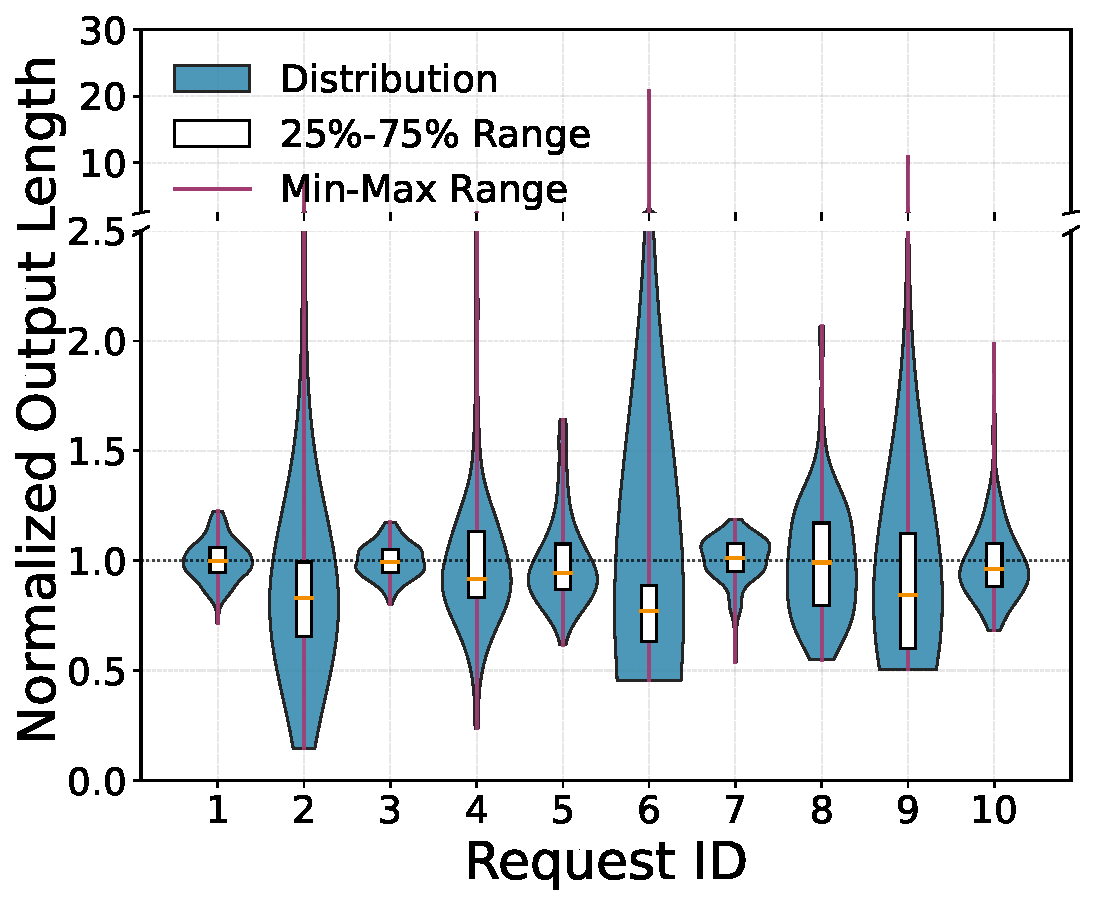
\includegraphics[width=0.45\linewidth]{figures/length_variation.pdf}
        \label{fig:background_uncertainty}
    }
    \hfill
    \subfigure[三个数据集请求在 H800 GPU 上单独剖析得到的散点图（执行时间，峰值显存占用）。]{
        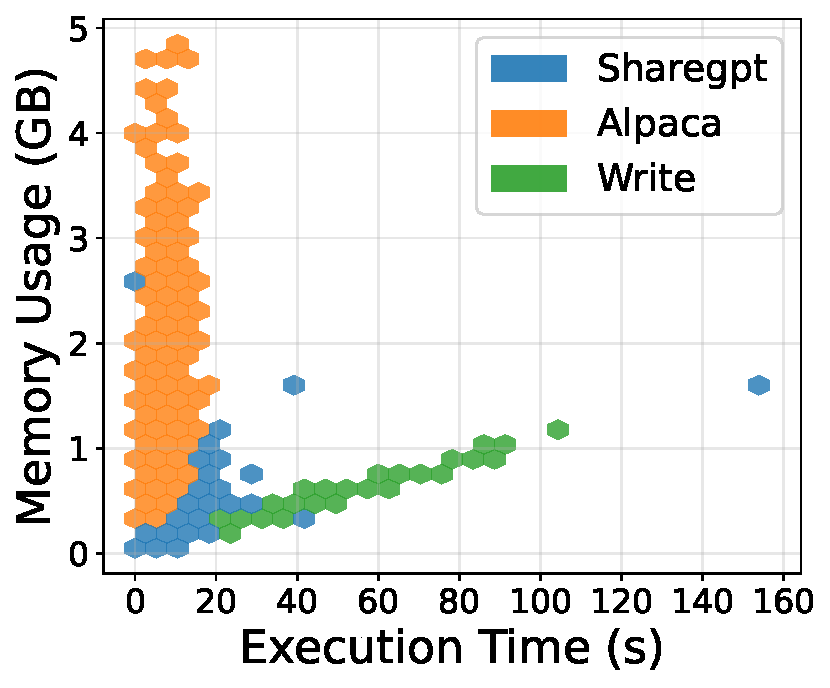
\includegraphics[width=0.45\linewidth]{figures/demand_hybridity.pdf}
        \label{fig:background_hybridity}
    }
    \caption{LLM 推理资源需求\emph{不确定性}与\emph{混合性}的实证证据。}
    \label{fig:background_uncertainty_and_hybridity}
\end{figure}

\phm{调度是 LLM 后端性能的关键。}
随着 LLM 需求爆发，来自不同用户的请求常在共享后端中处理，不同请求会竞争有限的计算与显存资源~\cite{Recasens2025Mind}。
为了提升用户体验，必须通过合理调度降低整体延迟。
尽管 LLM 有多种时延指标（TTFT、TPOT、TTLT），本文以 TTLT 为主，原因在于其综合性\footnote{
第一，TTLT 在智能体等场景中尤为关键：例如 LLM 驱动的机器人控制~\cite{chen2023typefly,wang2024llm}，下游动作通常要等到完整输出后才能启动。
第二，优化 TTLT 往往也会带来其他指标收益。
对于 TTFT，减少队首阻塞通常可直接改善首 token 时延（后续实验也将验证）；
对于 TPOT（统计中常定义为 TTLT 除以输出长度~\cite{wu2023fast,fu2024efficient}），降低 TTLT 也会带来比例改进。
}，这也与多项已有研究保持一致~\cite{shahout2024don,qiu2024efficient}。

\subsection{现有 LLM 调度器的局限}
\label{subsec:limitations}

现有文献已提出多种面向 LLM 推理的调度器。
针对需求不确定性，早期方法多为\emph{与需求无关}的启发式调度。
vLLM~\cite{kwon2023efficient}与 SGLang~\cite{zheng2024sglang}采用 FCFS，易受队首阻塞影响。
为缓解这一问题，FastServe~\cite{wu2023fast}使用\emph{多级反馈队列}（MLFQ），按固定服务配额周期性降低在途请求优先级，本质上近似 \emph{SRPT}，但会引入额外抢占开销。

发现上述不足后，近期调度器开始采用\emph{预测驱动}范式。
例如，SSJF~\cite{qiu2024efficient}利用微调 BERT-base 根据提示词预测输出长度，从而近似 SJF。
同时，Fu 等人~\cite{fu2024efficient}使用 OPT-125M 预测请求输出长度\emph{相对排序}而非绝对值。
近期 TRAIL~\cite{shahout2024don}则用 MLP 在迭代粒度持续预测输出长度，输入为特定 LLM 层特征嵌入。

\begin{figure}[t]
    \centering
    \subfigure[仅预测单一（分桶）值无法覆盖全部输出长度可能性；每个桶对应 100 token 区间。]{
        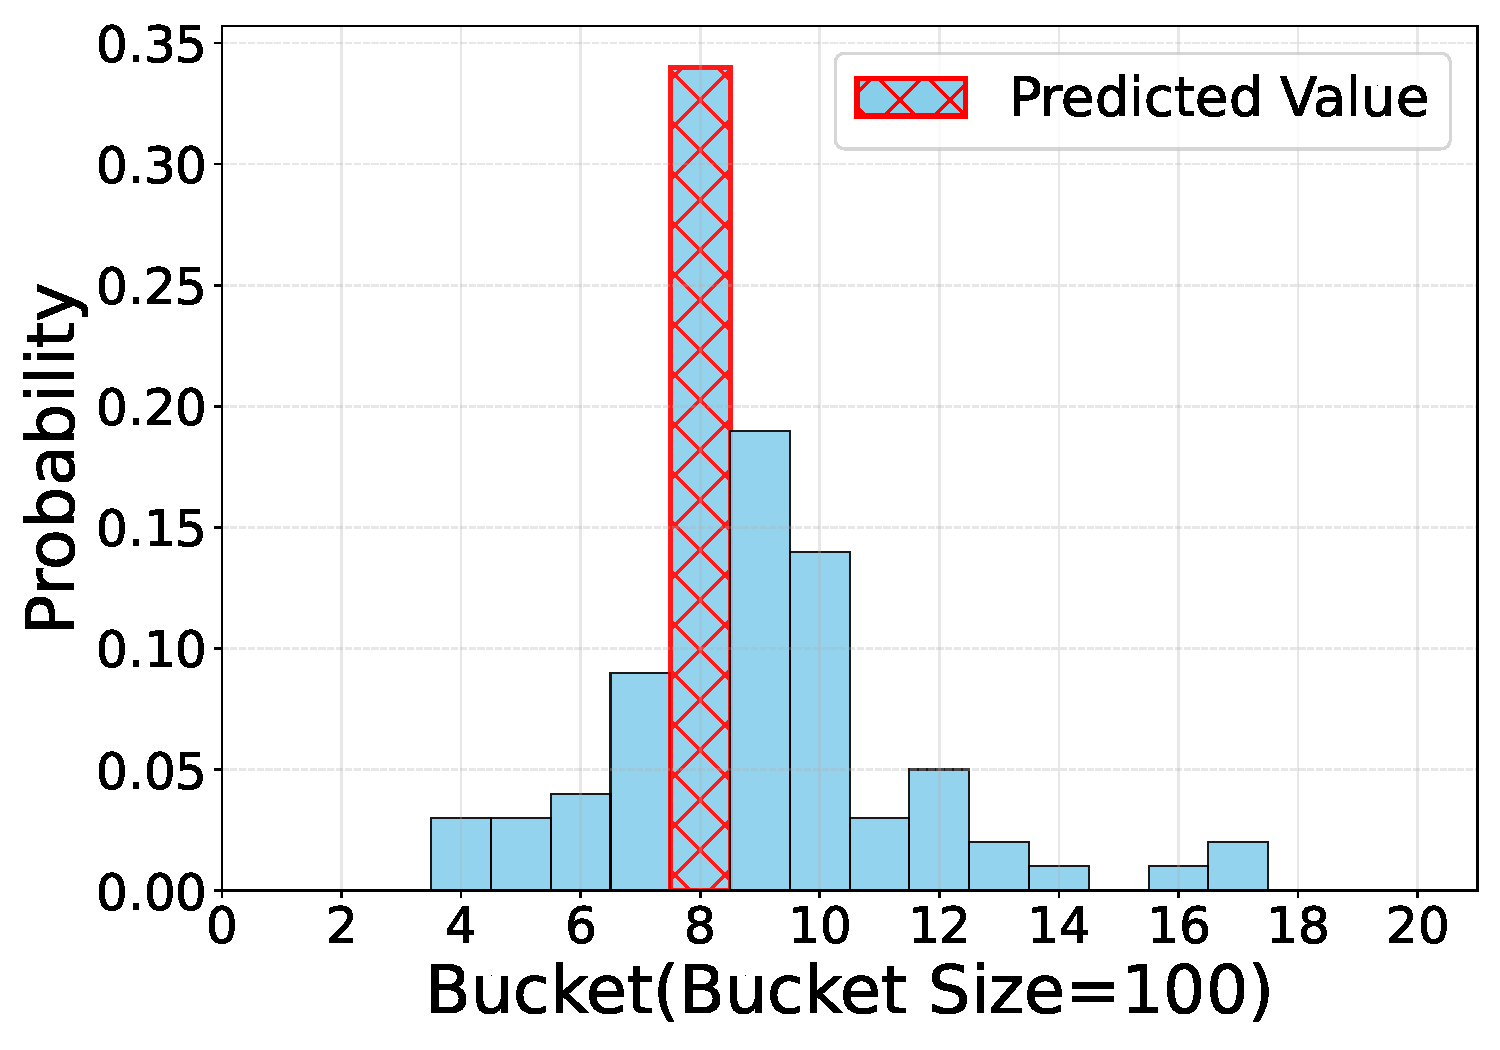
\includegraphics[width=0.53\linewidth]{figures/motivation_low_accuracy.pdf}
        \label{fig:low_prediction_accuracy}
    }
    \hfill
    \subfigure[受 KVCache 约束影响，仅优先短输出请求可能并非最优。]{
        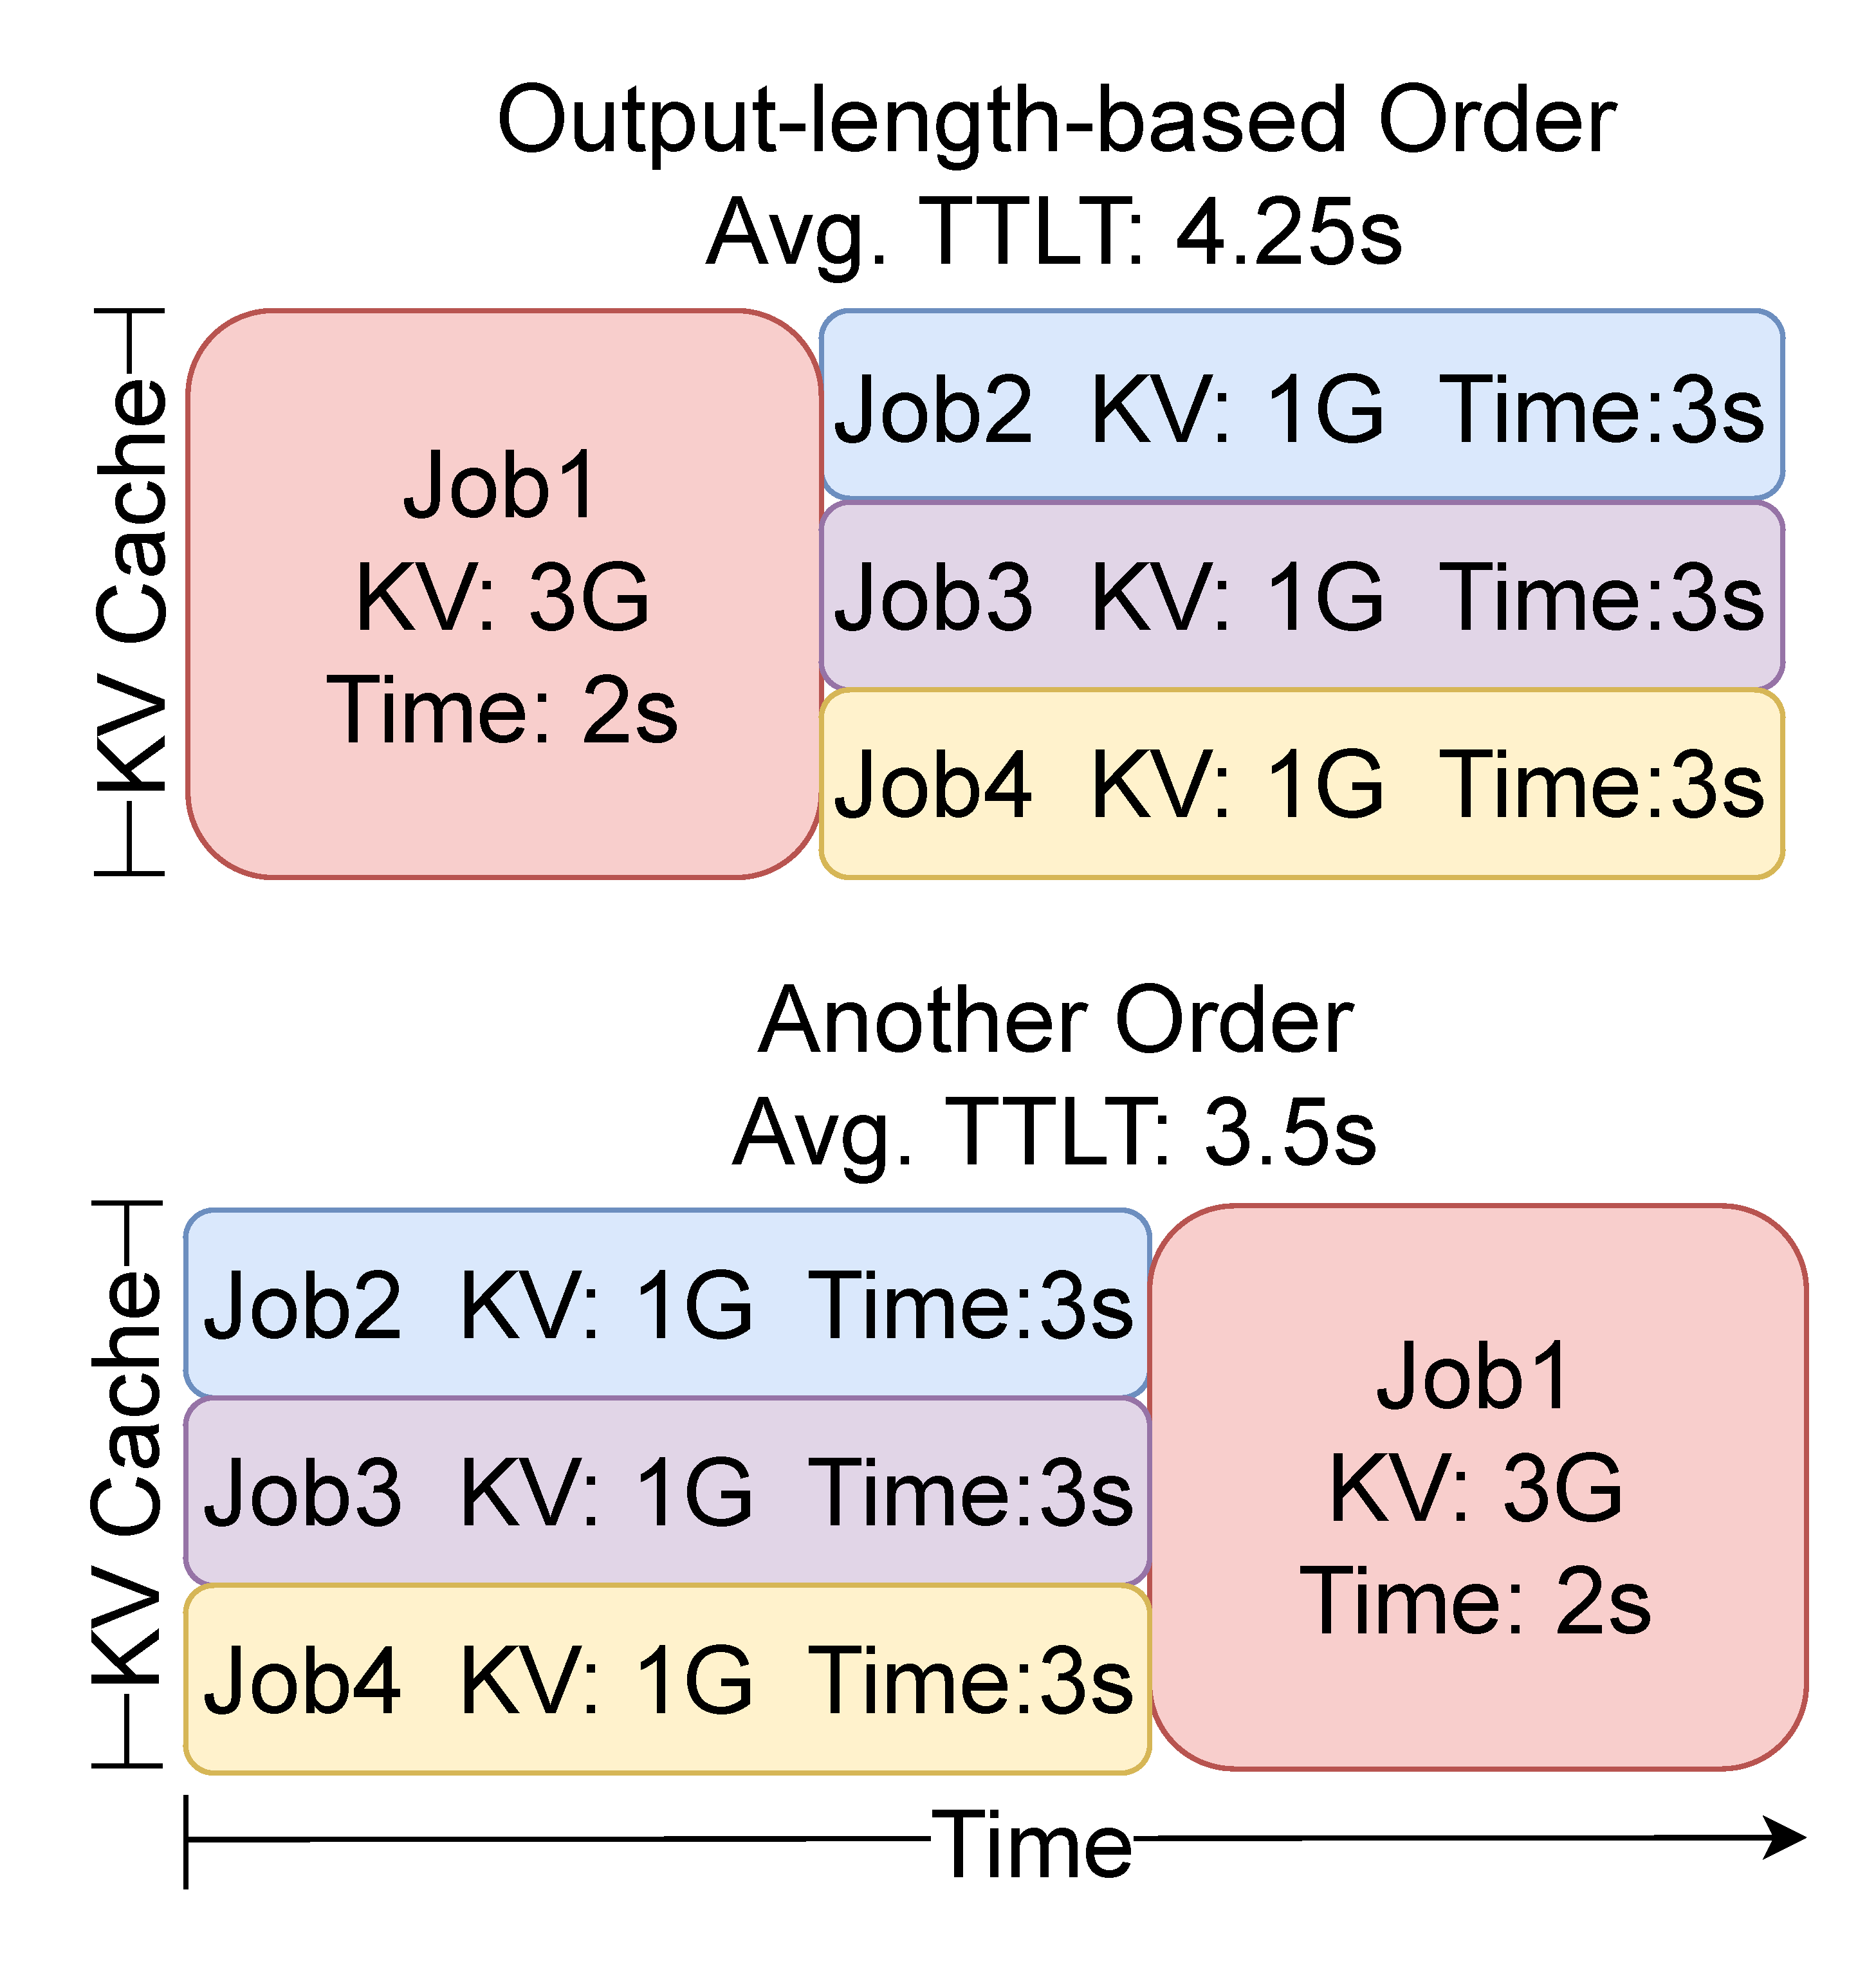
\includegraphics[width=0.37\linewidth]{figures/suboptimality_SJF.pdf}
        \label{fig:wrong_scheduling_order}
    }
    \caption{现有调度器在应对需求不确定性与混合性时的典型缺陷示例。}
    \label{fig:deficiencies}
\end{figure}

但上述预测型调度器在处理\emph{不确定性}方面仍不充分。
第一，它们的长度预测器通常需要较重的离线训练（微调常需 1 万+样本~\cite{jin2023s, fu2024efficient}），且在一个 LLM 上训练的模型难以直接迁移到另一个 LLM。
第二，这些预测器只输出\emph{单一值}，丢失了宝贵的分布信息。
实际上，不确定性是 LLM 推理的内生属性，单值预测很难准确。
如图~\ref{fig:low_prediction_accuracy} 所示，按~\cite{qiu2024efficient}方式使用 DistillBert 进行单值预测时，准确率仅 34.1\%（在 20 个桶中仅命中 1 个）。
而我们在第~\ref{subsec:gittins} 节将展示：保留长度分布信息可带来更优调度决策。
因此，在应对需求不确定性时，应设计一种\emph{免训练}且可直接预测输出长度\emph{分布}的方法。

同时，这些方法在处理需求\emph{混合性}方面也存在不足。
它们通常仅把计算时间（即输出 token 长度）作为服务代价，忽略了 GPU 显存占用。
事实上，输入和输出 token 都会占用 KVCache，因此即便输出长度相同，不同请求的显存代价也可能显著不同。
如图~\ref{fig:wrong_scheduling_order} 所示，当后端受显存瓶颈约束时，仅按“输出更短优先”排序可能是次优的。
因此，要处理 LLM 推理的混合性，必须联合考虑计算与显存两个维度。

综上，受需求不确定性与混合性影响，现有 LLM 调度器难以获得高整体效率。
下一节我们将提出新的高效调度器，分别从输出长度预测、代价建模与请求排队三方面进行优化。

%!TEX root = main_zh.tex
\section{SageSched 设计}
\label{sec:design}

\begin{figure}
    \centering
    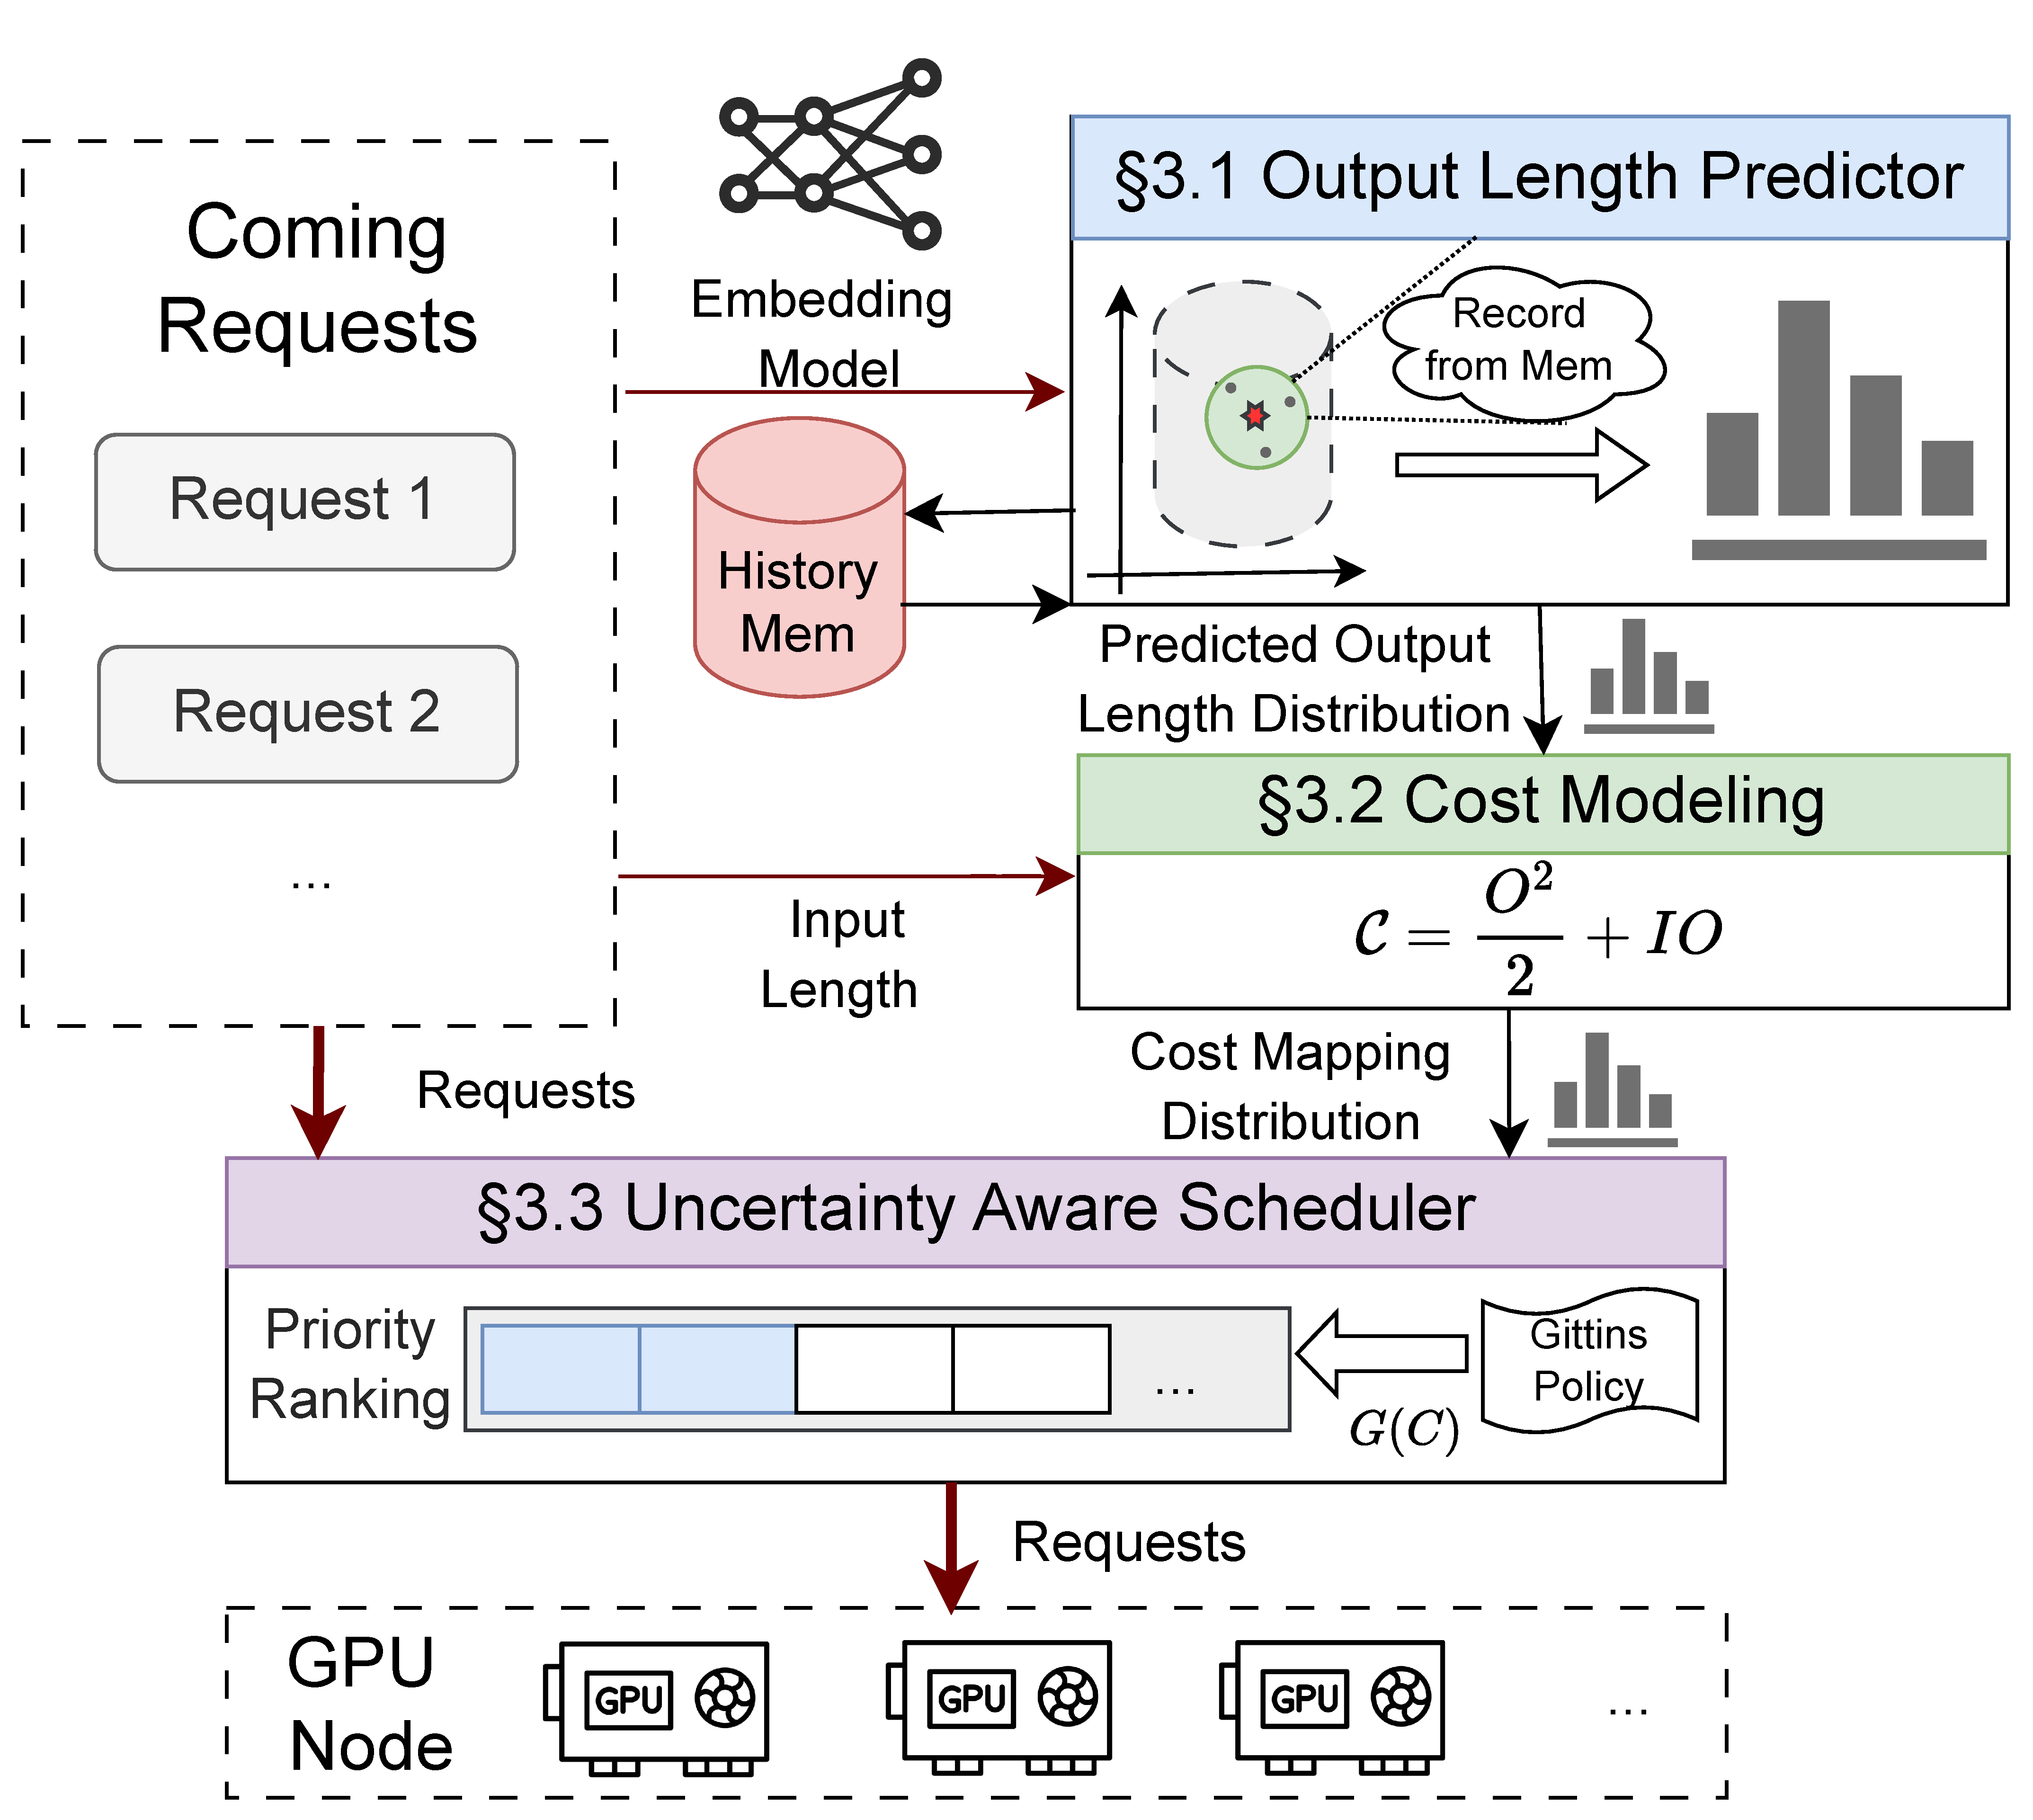
\includegraphics[width=0.8\linewidth]{figures/overview_new.pdf}
    \caption{\oursched 工作流程总览。}
    \label{fig:overview}
\end{figure}

本文提出 \oursched：一种通过正确处理需求不确定性与混合性来实现高效 TTLT 的新型 LLM 调度器。
整体流程如图~\ref{fig:overview} 所示。
对每个到达请求，\oursched 先使用轻量且准确的预测器估计其输出长度分布（第~\ref{subsec:predictor} 节）；
随后基于该分布并联合显存与计算资源，对请求总体服务代价进行建模（第~\ref{subsec:cost} 节）；
最后采用不确定性感知调度算法确定运行时排队顺序，以获得最优效率（第~\ref{subsec:gittins} 节）。

\subsection{语义感知的历史检索预测器}
\label{subsec:predictor}

如第~\ref{subsec:limitations} 节所述，鉴于 LLM 解码过程的内生不确定性，真正准确的预测应输出\emph{分布}而非\emph{单点数值}。
一个直接思路是改造现有预测模型（如 DistillBert~\cite{distilbert_docs}）的输出层，使其预测分布；本质上，该方法试图根据语义提示词直接\emph{逼近}最终生成效果。
但这类模型依然\emph{成本高}（训练代价大）且\emph{准确性有限}（生成过程难以直接近似）。

实际上，我们发现：给定提示词后，输出长度更适合通过\emph{参考近期历史中的相似请求}来预测，而非用微调模型直接模拟生成内部机制。
相比“直接模拟生成过程”，评估“提示词相似性”更容易。
同时，已有研究~\cite{gong2025past}表明，相邻滑动窗口内请求输出长度总体分布具有相对稳定性，这说明近期历史有很高参考价值。
因此，通过选取提示词相似的历史请求，我们有望得到\emph{更容易且更准确}的需求预测。

\begin{figure}[t]
    \centering
    \subfigure[从 \emph{Alpaca} 数据集中采样的 Prompt-1]{
        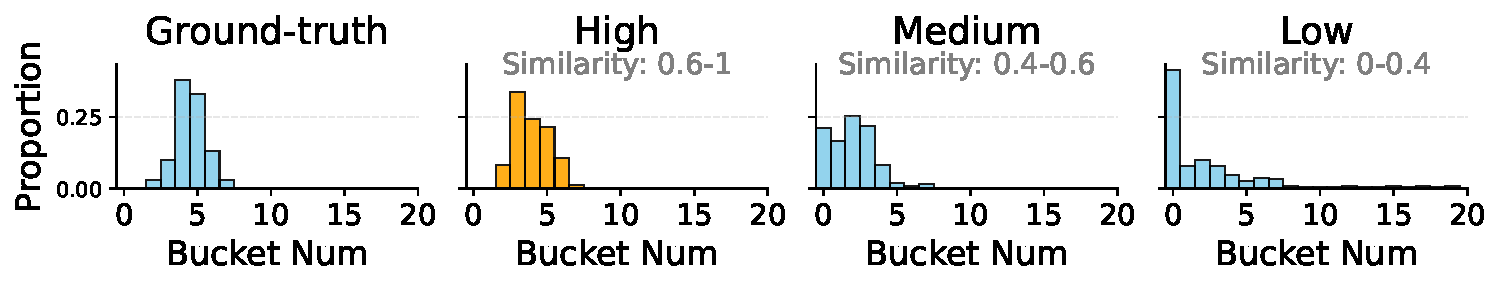
\includegraphics[width=0.9\linewidth]{figures/all_distributions_sample_39.pdf}
        \label{fig:correlation-1}
    }
    \hfill
    \subfigure[从 \emph{Write} 数据集中采样的 Prompt-2]{
        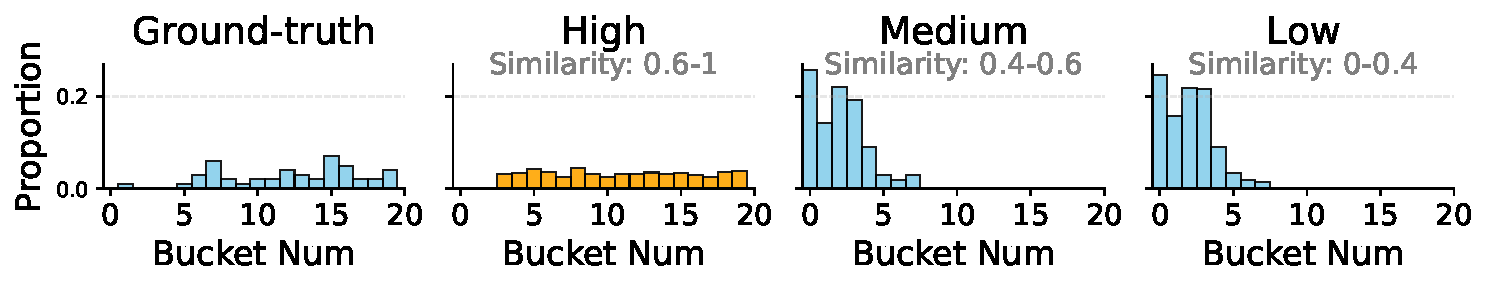
\includegraphics[width=0.9\linewidth]{figures/all_distributions_sample_57.pdf}
        \label{fig:correlation-2}
    }
    \caption{请求输出长度分布可由提示词相似度更高的历史请求更好地逼近。}
    \label{fig:prompt-correlation}
\end{figure}

为验证该点，我们实证分析提示词相似度与输出长度分布相似度之间的相关性。
我们分别从 Alpaca 与 Write 数据集采样一个提示词。
对于每个提示词，先重复推理 100 次，得到其输出长度分布作为待预测真值；
再按与该提示词的相似度将历史请求分为三组，其中相似度通过两请求提示词嵌入的\emph{余弦相似度}计算。
图~\ref{fig:prompt-correlation} 显示，两组实验都存在明确相关性：\emph{相似度更高}的历史组，其分布曲线形状与目标分布\emph{更接近}。

基于以上观察，我们提出\emph{语义感知的历史检索预测器}，融合\emph{提示词内容}与\emph{历史执行结果}，直接预测输出长度分布。
具体实现上，我们维护近期请求的推理记录（提示词与输出长度）。
对每个新请求，检索\footnote{历史窗口大小设为 10,000，按 FIFO 持续更新。若高相似样本不足（如冷启动阶段），我们使用公开数据集请求补充候选集。向量检索采用 \emph{FAISS IndexFlat}~\cite{faiss_meta}，通常耗时低于 1 ms。}
与其提示词足够相似的历史请求（默认阈值 0.8），并将这些样本的输出长度分布作为预测结果。
该方法无需微调模型，对不同 LLM 均具通用性，也无需直接模拟复杂生成过程。
因此可以同时实现轻量与准确的分布预测。

\subsection{基于资源瓶颈的代价建模}
\label{subsec:cost}

有了上述预测方法后，我们可得到每个请求的输出长度分布。
但如第~\ref{subsec:limitations} 节所述，受需求混合性影响，直接用输出长度作为服务代价并不充分。
本节目标是建立一个同时考虑计算与显存的综合代价模型。

对于多资源代价建模，关键先判断真实瓶颈资源，因为它决定后续分析路径。
在实际中，LLM 服务后端可能处于\emph{计算瓶颈}或\emph{显存瓶颈}，这取决于运行时负载特征。
具体地，图~\ref{fig:diverse_bounds} 展示了在 H100 上，随 batch 增大时解码步的计算与显存关系。\footnote{图~\ref{fig:bounds_and_observations} 中 GPU 利用率通过“实际 TFLOPs/峰值 TFLOPs”估算，CUDA 时间使用 \texttt{torch.profiler} 测量。}
我们将序列长度（输入长度 + 当前已生成长度）分别固定为 50 与 1000。
长序列更偏显存密集：短序列下，达到显存上限前 GPU 利用率已较高；长序列下，显存先满而 GPU 利用率尚未充分上升。
注意，某类资源代价仅在该资源成为瓶颈时才决定性能。
因此我们分别讨论两种状态下的代价刻画。

\begin{figure}[t]
    \centering
    \subfigure[batch 增大时 GPU 利用率与 KVCache 占用关系。]{
        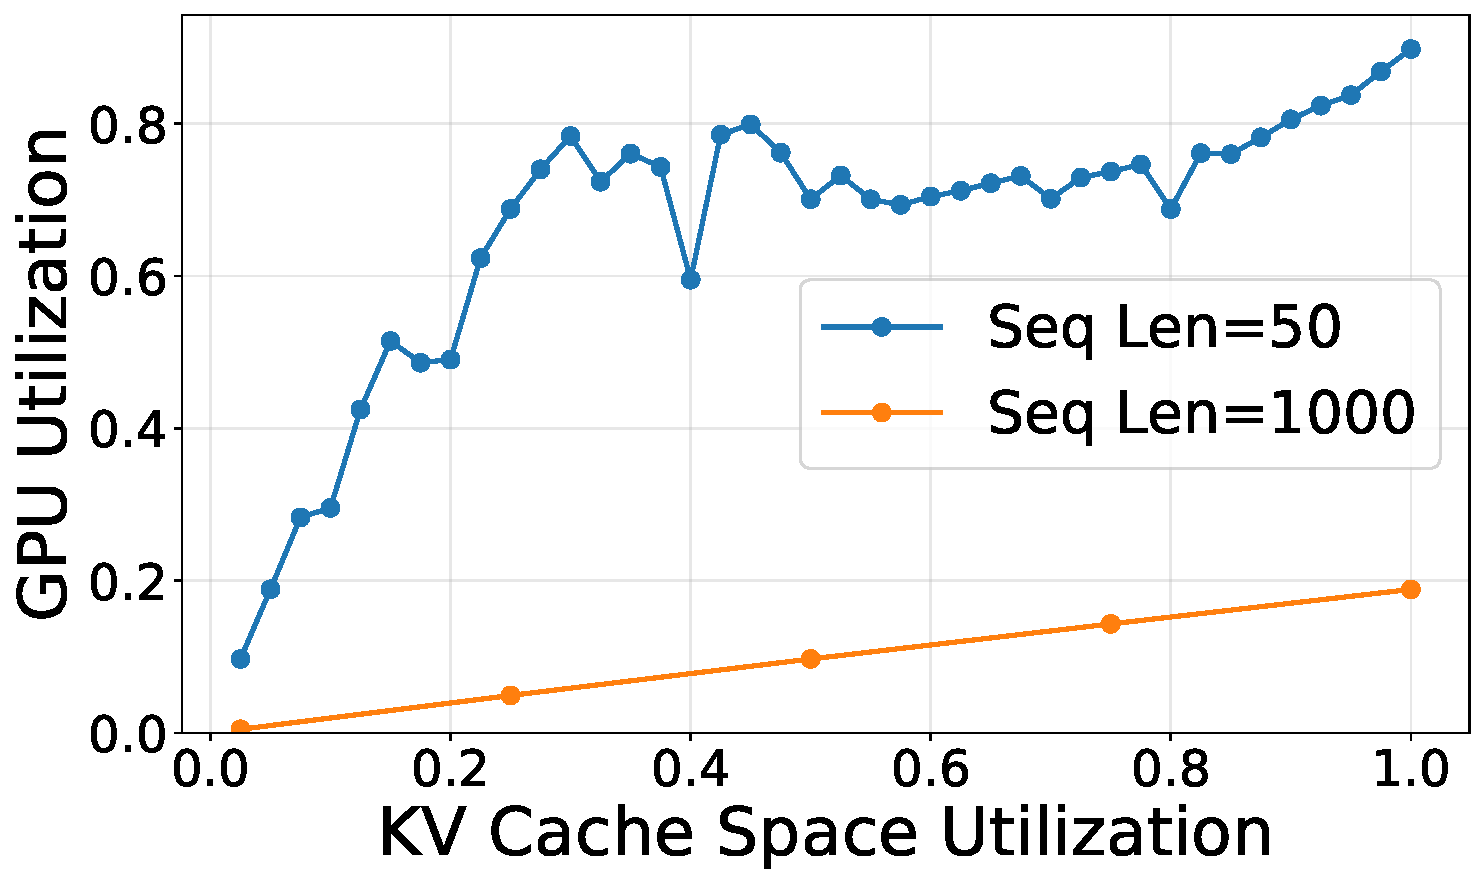
\includegraphics[width=0.45\linewidth]{figures/two_workloads_varying_batch.pdf}
        \label{fig:diverse_bounds}
    }
    \hfill
    \subfigure[解码过程中每步注意力计算时间的变化。]{
        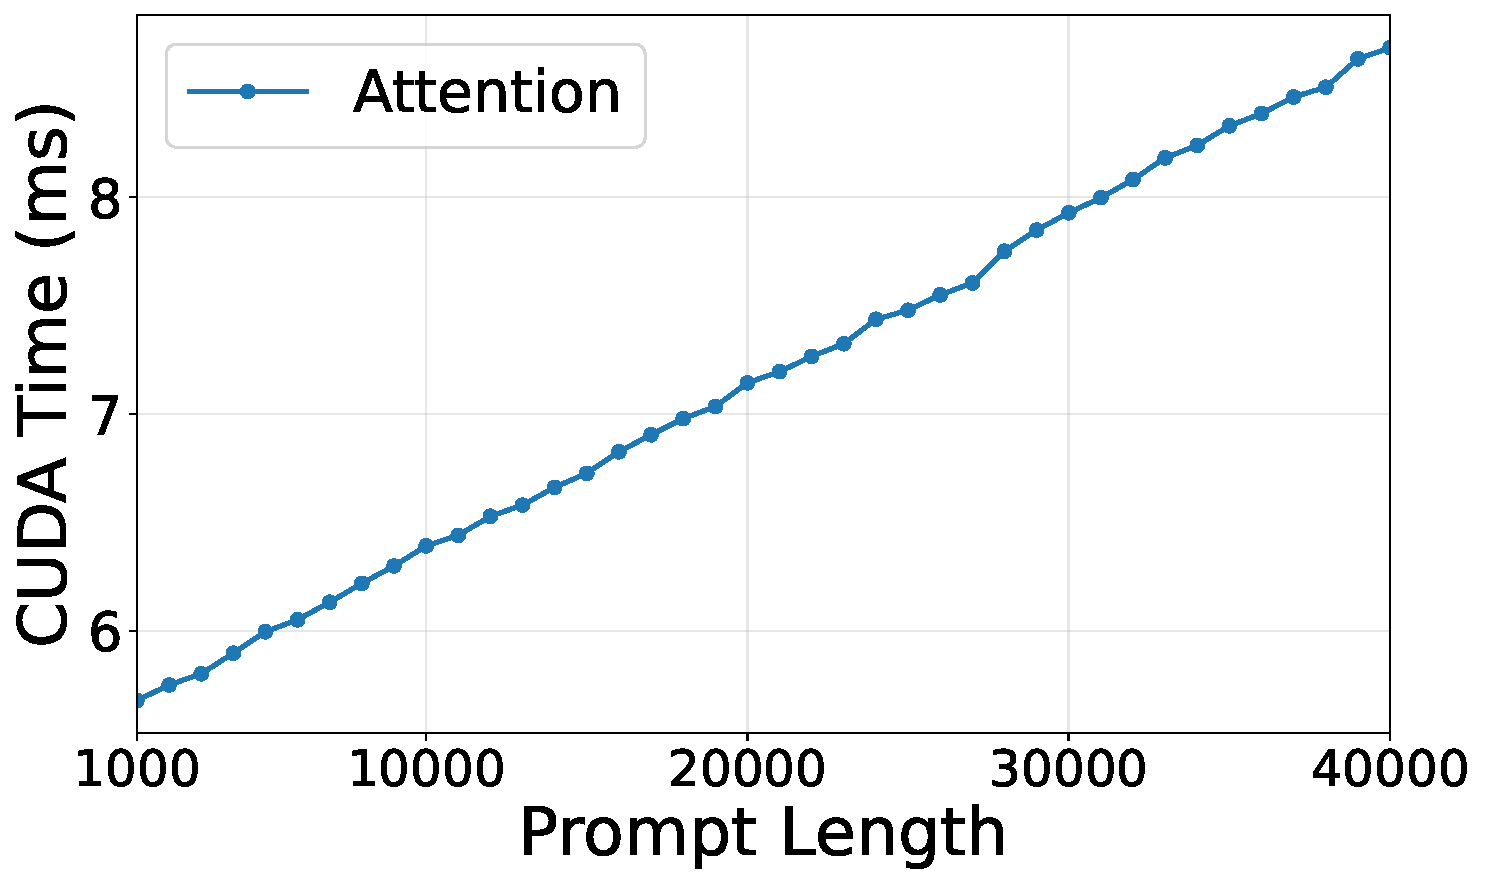
\includegraphics[width=0.45\linewidth]{figures/simple_module_analysis_attention.pdf}
        \label{fig:compute_cost}
    }
    \caption{瞬时资源瓶颈测量，以及解码阶段计算代价特征。实验均在 H800 + Qwen3-32B 上完成。}
    \label{fig:bounds_and_observations}
\end{figure}

先看\emph{显存瓶颈}场景。
此时，请求 KVCache 占用是建模关键因素——KVCache 越省，可并发服务的请求越多（且在 GPU 利用率不高时，提高并发不会显著增加迭代时长）。
因此在显存瓶颈下，应主要考虑请求生命周期内的累计 KVCache 占用。
设推理输入（提示词）长度和输出长度分别为 $I$、$O$，其总服务代价可表示为
$\mathcal{C}_M=\sum_{l=I}^{I+O}l*U_{MT}=(\frac{O^2}{2}+IO)U_{MT}$，
其中 $U_{MT}$ 表示单位\emph{显存-时间}乘积（即单 token 在单步中的 KVCache 占用量）。

再看\emph{计算瓶颈}场景。
该情况下，KVCache 占用不再是主要约束，我们只需量化请求全生命周期的总计算量。
图~\ref{fig:compute_cost} 测得：不同解码步下，注意力模块（Transformer 的关键计算部分）每步计算时间近似与累计序列长度线性相关。\footnote{本文聚焦\emph{解码}阶段资源消耗；随着\emph{推理型 LLM}~\cite{cai2025r}普及，解码阶段通常主导 TTLT。除线性增长的注意力时间外，还存在与序列长度无关的近似常量 FFN 时间（以及 CUDA 启动等小开销），但在长解码或大 batch 下可被显著摊薄，因此此处略去。}
由此可得总计算代价
$\mathcal{C}_C=\sum_{l=I}^{I+O}l*U_{CT}=(\frac{O^2}{2}+IO)U_{CT}$，
其中 $U_{CT}$ 为单位\emph{计算-时间}乘积（单 token 在单步平均计算量）。

综合上述分析，计算代价与显存代价共享同一函数形式（仅单位不同，不影响请求间相对排序）。
因此实践中可采用统一代价模型（无需显式切换瓶颈模式）：
$\mathcal{C}=\frac{O^2}{2}+IO$。
尽管跨资源形式一致，我们的方法与既有建模显著不同——例如~\cite{qiu2024efficient,fu2024efficient,shahout2024don}仅用 $O$，或~\cite{sheng2024fairness}采用 $I$ 与 $O$ 的简单加权和。
我们在第~\ref{sec:cost modeling} 节实验中将验证该建模方式的优越性。

\subsection{不确定性感知请求调度}
\label{subsec:gittins}

借助上述预测与建模，我们可在请求到达时得到其代价分布（可缓解但无法完全消除不确定性）。
接下来需要一个不确定性感知调度算法，以达到理论最优 TTLT。

\begin{figure}[t]
    \centering
        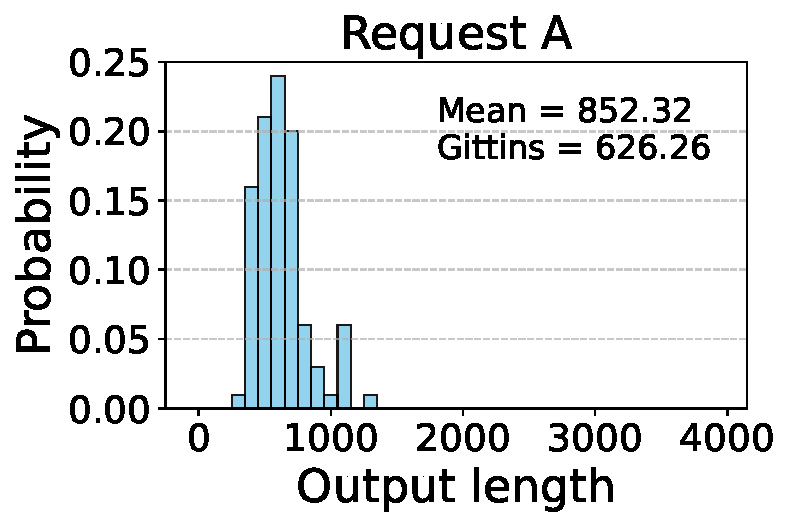
\includegraphics[width=0.45\linewidth]{figures/motivation_gittins_example_A.pdf}
        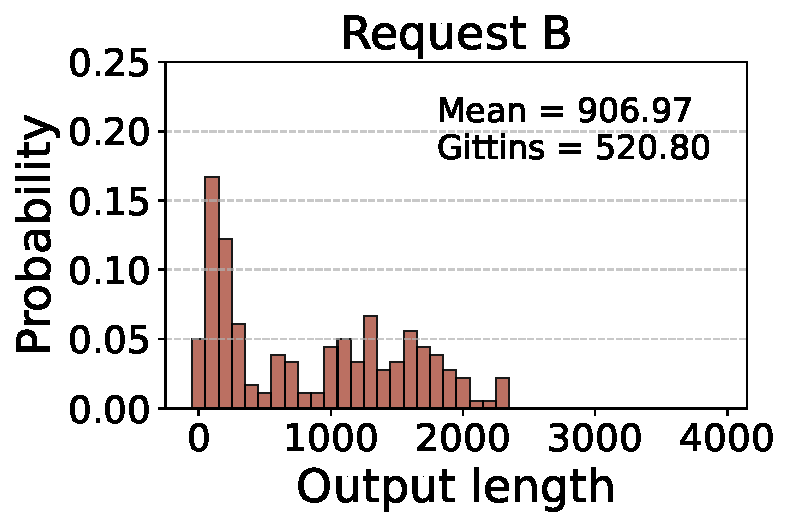
\includegraphics[width=0.45\linewidth]{figures/motivation_gittins_example_B.pdf}
    \caption{均值优先排序的缺陷示例。尽管请求 B 的均值更大，但由于其分布形状不规则，先服务 B 在平均 TTLT 上反而可能更优。}
    \label{fig:gittins}
\end{figure}

排队时，需要从每个请求的代价分布中计算合适调度指标；如图~\ref{fig:gittins} 所示，均值并非最优。
我们注意到，选择“当前优先服务哪个请求”可类比为\emph{多臂老虎机}问题中的“选择哪个臂”~\cite{mahajan2008multi}：
请求代价分布本质上描述了“继续分配资源后完成请求的收益分布”。
对于“收益随机但分布已知”的老虎机问题，文献已证明\emph{Gittins 策略}~\cite{gittins1979bandit}可达理论最优。

具体地，给定请求代价分布 $\mathcal{D}$，其 Gittins 指数定义为
$G(\mathcal{D})=\operatorname*{inf}_{\Delta>0,X\sim\mathcal{D}}{\frac{\operatorname{E}[\operatorname*{min}\{X,\Delta\}]}{\operatorname*{P}(X\leq\Delta)}}$；
调度时优先选择 Gittins 指数更小的请求。
其中，$\operatorname{E}[\operatorname*{min}\{X,\Delta\}]$ 表示给定服务预算 $\Delta$ 时的期望服务消耗，$\operatorname*{P}(X\leq\Delta)$ 表示在该预算内完成请求的概率；因此 $G$ 刻画了该请求可达到的最小摊销代价。
已有理论证明，基于 Gittins 指数（而非分布均值）调度可最小化平均延迟（TTLT）~\cite{gittins1989multiprocessor}。
图~\ref{fig:gittins} 也展示了其直观效果：该策略会优先处理“近期更可能完成”的请求。

此外，请求开始执行后，其 Gittins 指数应在运行时动态更新。
TRAIL~\cite{shahout2024don}与 FastServe~\cite{wu2023fast}都表明，启用抢占对优化平均 TTLT 很重要（在交换计算重叠、KVCache 预取等技术支持下，开销可忽略）。
理想做法是每一步都依据\emph{剩余}代价分布刷新指数。
但逐步刷新在实践中成本过高，且易引发抖动（指数接近的请求可能频繁互换优先级）。
因此我们将每个请求代价范围划分为多个桶（默认 10 个），仅在桶边界刷新其 Gittins 指数。
这样可在调度时效与系统稳定性之间取得平衡。

%!TEX root = main_zh.tex
\section{实验评估}
\label{sec:eval}

\subsection{实验设置}
\phm{硬件平台。}
在测试床实验中，我们分别以 Llama3.1-8B~\cite{llama3_1_8b_instruct} 和 Qwen3-32B~\cite{qwen3_32b} 作为后端模型。
其中 Llama3.1-8B 部署在 A40-PCIe-48GB 服务器上，Qwen3-32B 部署在 H800-PCIe-96GB 服务器上。
此外，我们还构建了可扩展至 {64 张 GPU} 的模拟器，用于评估 \oursched 的可扩展性。

\phm{工作负载。}
实验使用与~\cite{hu2024inference}一致的三类推理数据集：SharedGPT~\cite{sharegpt_vicuna_unfiltered_2025}、Alpaca-Summarization~\cite{alpaca_pubmed_summarization_2025} 与 Document-Write~\cite{write_doc_sft_v1_2025}。
这些数据集特征已在图~\ref{fig:background_hybridity} 中展示。
请求提交间隔采用不同 $\lambda$ 参数的泊松分布，以覆盖不同任务到达速率。

\phm{对比方法。}
我们将 \oursched 与多个代表性基线比较：FCFS~\cite{kwon2023efficient}、FastServe~\cite{wu2023fast}、SSJF~\cite{qiu2024efficient}、LTR~\cite{fu2024efficient} 和 TRIAL~\cite{shahout2024don}。
这些方法已在第~\ref{subsec:limitations} 节介绍，实验中均采用其默认超参数。
此外，\oursched 默认设置为：预测器选择阈值 0.8，Gittins 分析桶大小 200。

\phm{评测指标。}
如第~\ref{subsec:problem} 节所述，我们以平均 TTLT 作为核心指标。
同时也报告平均 TTFT（首 token 时间）。

\subsection{端到端实验}

\begin{figure}[t]
    \centering
    \subfigure[Llama3.1-8B]{
        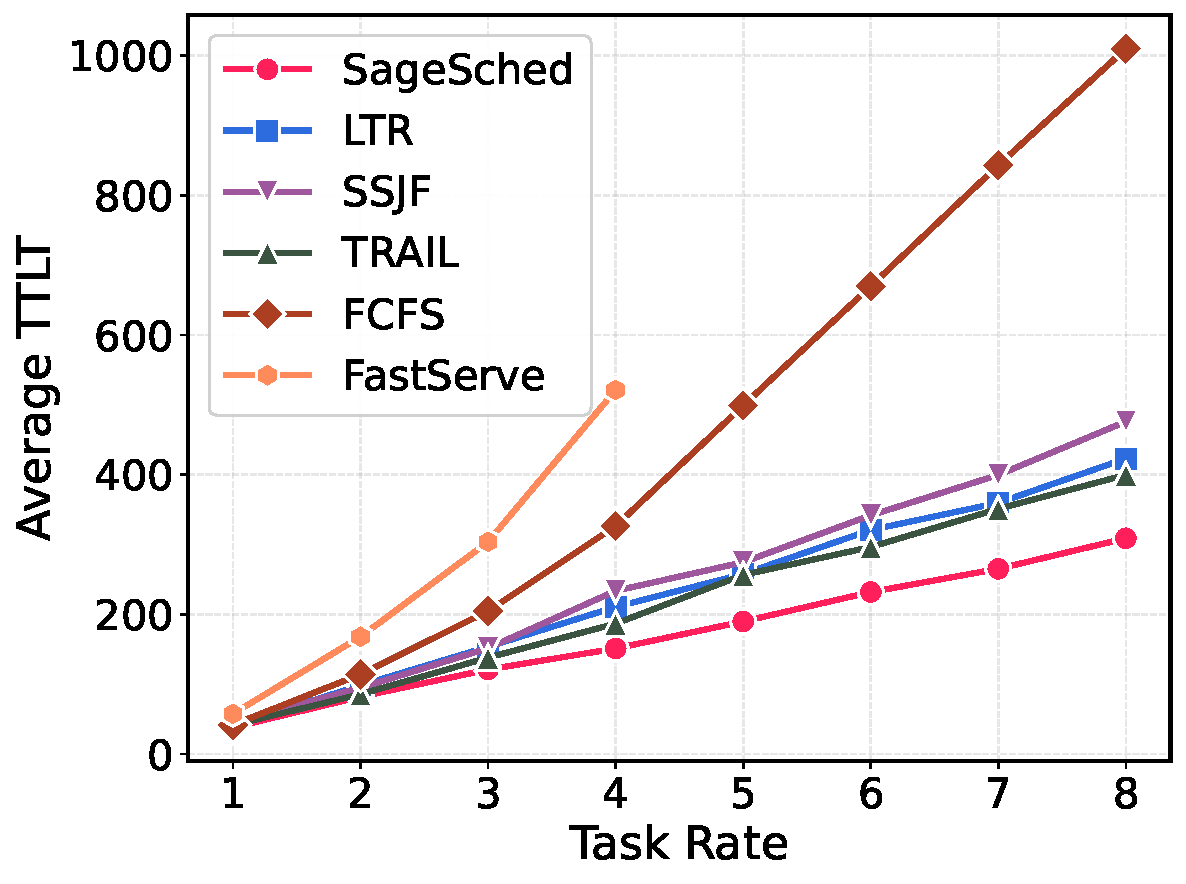
\includegraphics[width=0.45\linewidth]{figures/ttlt_plot_8b.pdf}
        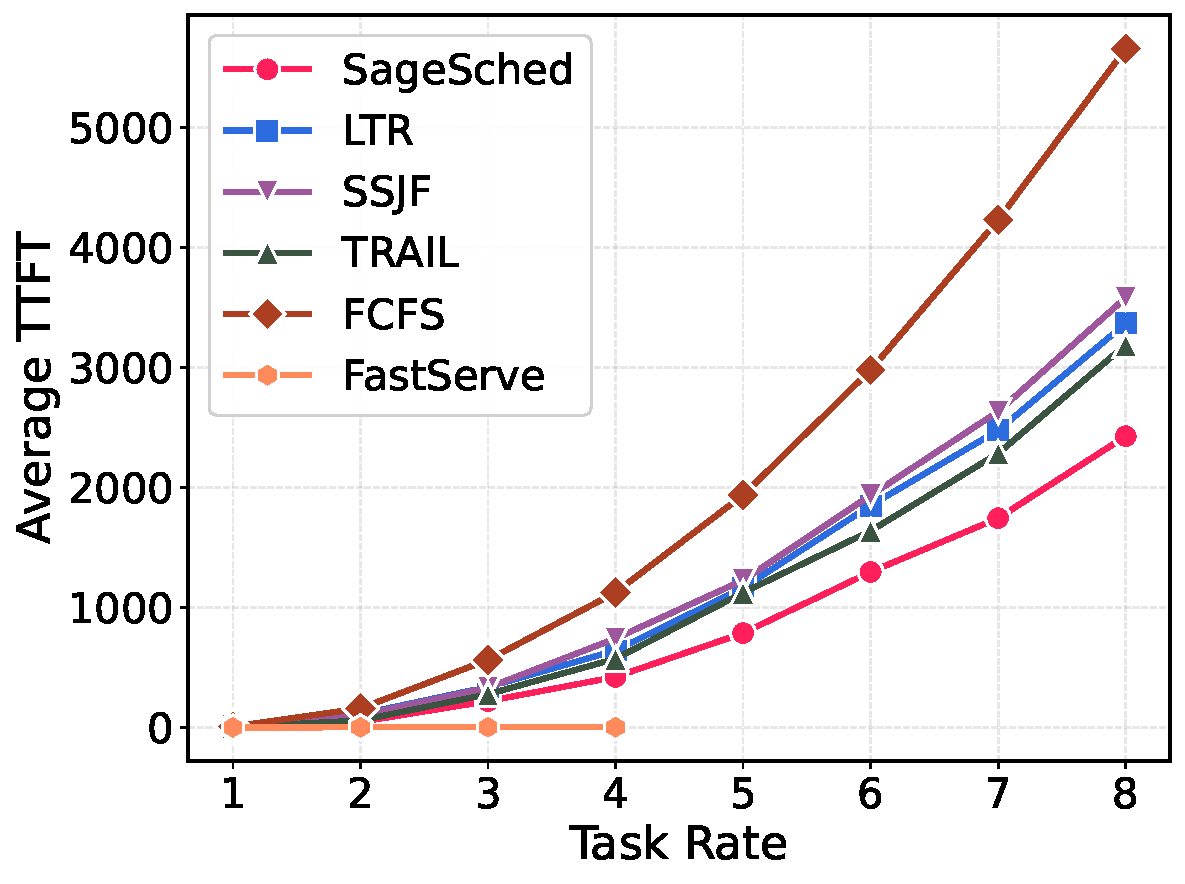
\includegraphics[width=0.45\linewidth]{figures/ttft_plot_8b.pdf}
        \label{fig:e2e 8b ttft}
    }

    \subfigure[Qwen3-32B]{
        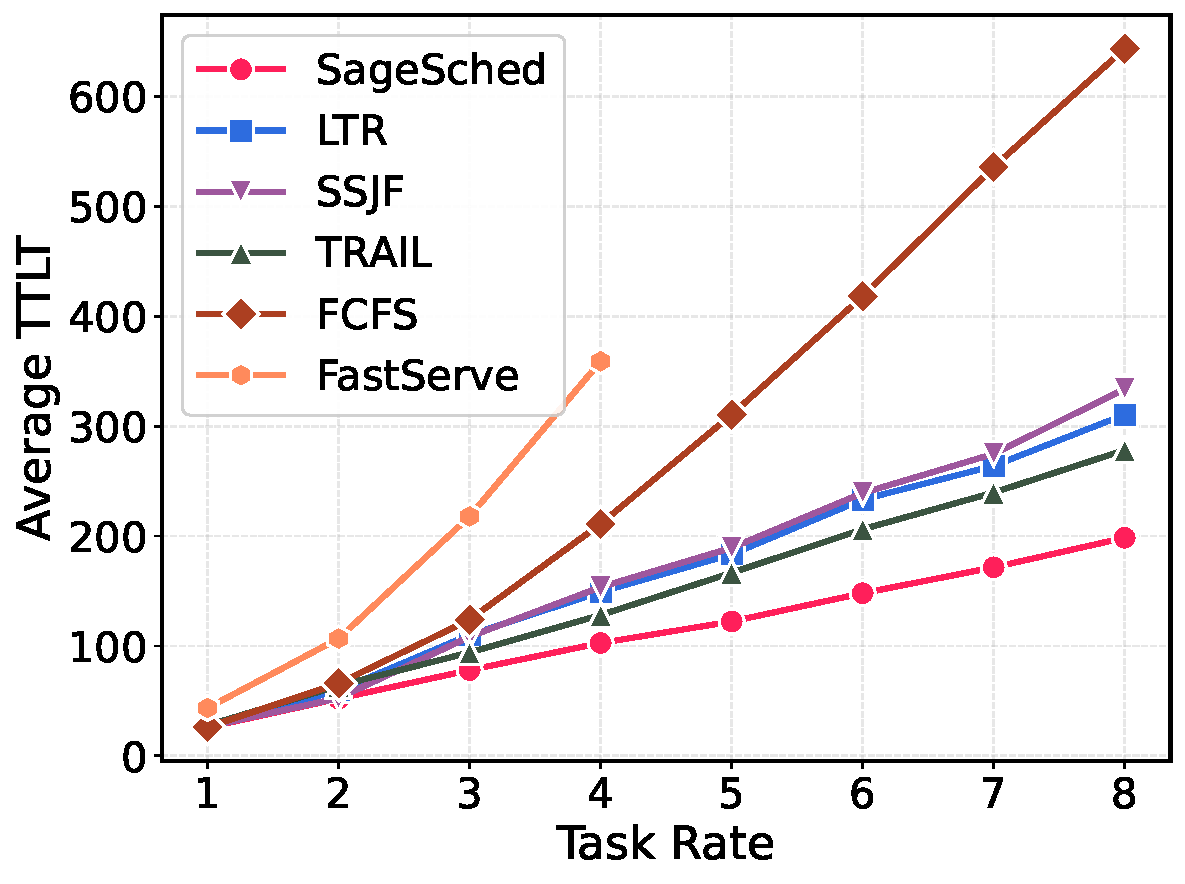
\includegraphics[width=0.45\linewidth]{figures/ttlt_plot_32b.pdf}
        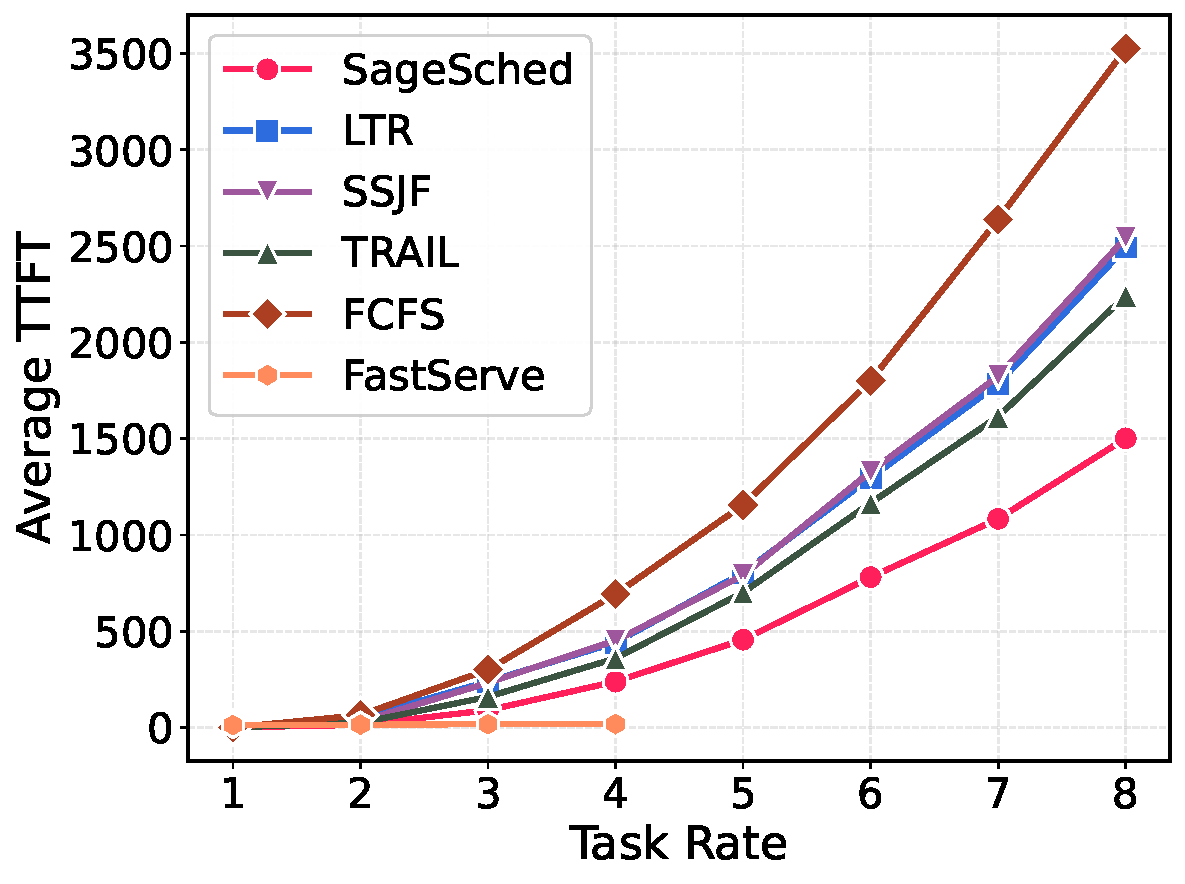
\includegraphics[width=0.45\linewidth]{figures/ttft_plot_32b.pdf}
        \label{fig:e2e 32b ttft}
    }

    \caption{混合数据集下的端到端性能。}
    \label{fig:e2e}
\end{figure}

\phm{混合数据集请求实验。}
端到端实验中，我们先将三个数据集合并，再随机提交请求，并在不同任务速率下评测。
如图~\ref{fig:e2e} 所示，\oursched 在所有设置下都取得了最佳 TTLT 效率。
例如，在 Qwen3-32B 上、请求速率为 8 RPS 时，\oursched 相比次优方法 TRAIL 的 TTLT 进一步降低 28.7\%。
竞争越激烈，这一优势越明显，因为 \oursched 能更稳定地利用不确定性与混合性信息计算更优排队顺序。

对于 TTFT，虽然并非本文主要目标，但图~\ref{fig:e2e} 显示 \oursched 同样表现良好，因为它能够有效缓解队首阻塞。
特别地，FastServe 虽然通过优先新到请求获得了最优 TTFT，但其 MLFQ 交替执行机制导致 TTLT 明显劣于其他方法。
因此，\oursched 是少数能在 TTLT 与 TTFT 上同时保持优异表现的调度器。

\begin{figure}
    \centering
    
\includegraphics[width=1\linewidth]{figures/end_to_end.pdf}
    \caption{分别在各单一数据集上的端到端性能。}
    \label{fig:single_dataset}
\end{figure}

\phm{单数据集请求实验。}
回顾图~\ref{fig:background_hybridity}，三类数据集的输入/输出长度分布差异明显。
因此我们分别在每个数据集上独立评测，结果见图~\ref{fig:single_dataset}。
可以看到，\oursched 在每个数据集上都稳定最优。
尤其在 Alpaca（摘要）数据集上优势最大：该数据集请求通常输入较长，现有仅基于输出长度的建模方法在此场景代价估计误差更大。

\subsection{微观深入分析}

本节进一步验证 \oursched 各组成模块的有效性。
除非特别说明，默认设置与图~\ref{fig:e2e}一致（RPS=8）。

\subsubsection{预测器设计的优越性}

针对传统输出长度预测器不足，我们在第~\ref{subsec:predictor} 节提出了\emph{语义感知历史预测器}。
这里从端到端 TTLT 角度验证其必要性。
具体引入两个对照预测器：
(1) \emph{语义无关的历史预测器}——按输入长度相近筛选历史请求并预测分布（筛选流程与我们一致）；
(2) \emph{语义感知的 LLM 预测器}——仍使用~\cite{qiu2024efficient}中的 DistillBert，但为输出分布，去除 \texttt{logits.argmax} 层。
图~\ref{fig:ablation_prediction} 给出不同预测器下 \oursched 的表现。
结果表明，我们的语义感知历史预测器因分布预测更准确，从而实现最佳 TTLT。

同时，在训练与推理开销方面，我们的方法也优于替代方案。
第一，我们完全免除了训练成本；而 LLM 预测器需数小时构造训练集并额外花费数十分钟微调。
第二，我们方法的单请求平均预测延迟低于 0.5 ms（语义嵌入提取 0.22 ms，向量检索 0.15 ms）；LLM 预测器约为 3.6 ms。
这些结果共同证明：我们的预测器兼具轻量与准确。

\begin{figure}
    \centering
    \begin{minipage}[t]{0.47\linewidth}
        \centering
        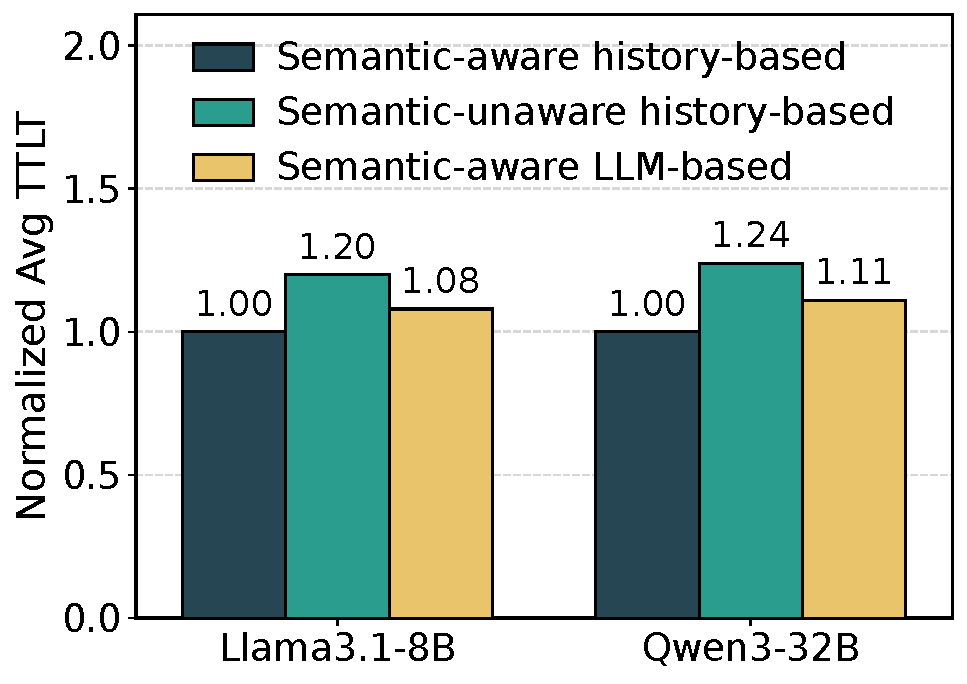
\includegraphics[width=\linewidth]{figures/ablation_on_influence.pdf}
        \caption{不同输出长度预测方法的性能对比。}
        \label{fig:ablation_prediction}
    \end{minipage}
    \hfill
    \begin{minipage}[t]{0.47\linewidth}
         \centering
        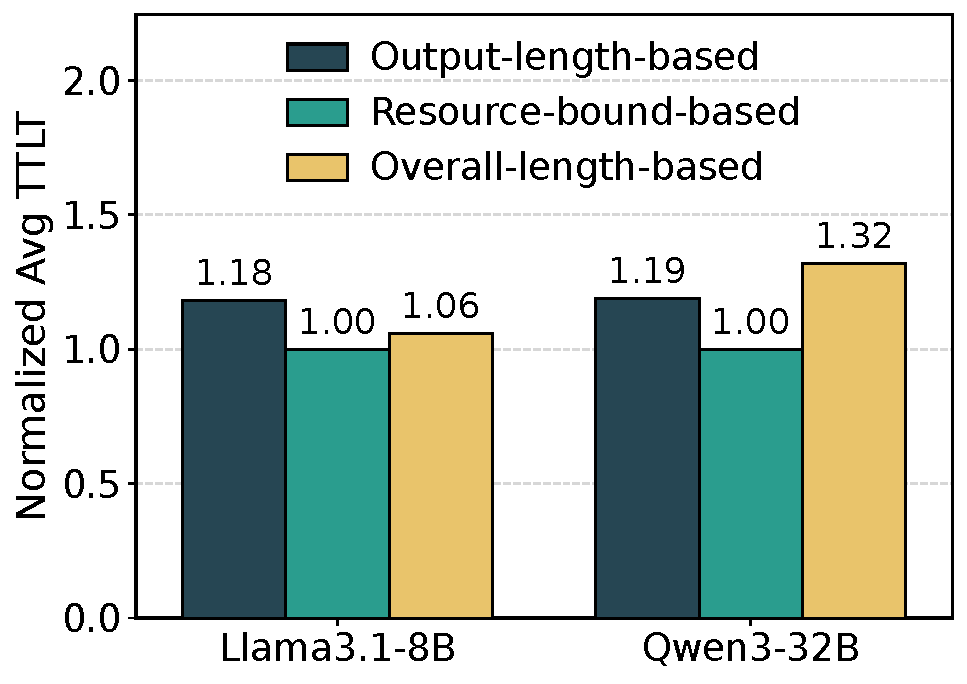
\includegraphics[width=\linewidth]{figures/ablation_on_cost.pdf}
        \caption{不同服务代价建模方法的性能对比。}
        \label{fig:ablation_cost}
    \end{minipage}
    \hfill
\end{figure}

\subsubsection{代价建模方法的优越性}
\label{sec:cost modeling}

在第~\ref{subsec:cost} 节中，我们分别分析计算瓶颈与显存瓶颈后提出了\emph{资源瓶颈驱动建模}方法。
为验证其必要性，我们将其替换为两种常见方案：
(1) \emph{基于输出长度建模}——直接以输出长度作为代价~\cite{shahout2024don,qiu2024efficient}；
(2) \emph{基于总长度建模}——将输入与输出长度加权求和（与~\cite{sheng2024fairness}一致，输出长度权重设为 2）。
图~\ref{fig:ablation_cost} 展示了不同建模方法下整体 TTLT。
结果确认了资源瓶颈驱动建模的必要性。

\subsubsection{调度策略的优越性}

回顾第~\ref{subsec:gittins} 节，我们的不确定性感知调度包含两项关键技术：
\emph{基于 Gittins 指数排序}与\emph{运行时 Gittins 指数刷新}。
这里分别评估其贡献，并检验在预测不准确时的鲁棒性。
具体地，我们加入两个额外基线：
(1) \emph{Mean}——按代价分布\emph{均值}排序；
(2) \emph{Gittins}$-$——使用 Gittins 策略，但不在桶边界及时刷新指数。
此外，对每种调度器我们还构造\emph{不准确预测}场景：将原始分布与\emph{均匀分布}按 4:1 融合注入噪声。
图~\ref{fig:ablation_gittins} 表明，Gittins 排序与运行时刷新都能显著提升 TTLT；同时，相比其他方法，注入噪声对我们基于 Gittins 的算法影响更小。

\begin{figure}[t]
    \centering
    \begin{minipage}[t]{0.47\linewidth}
        \centering
        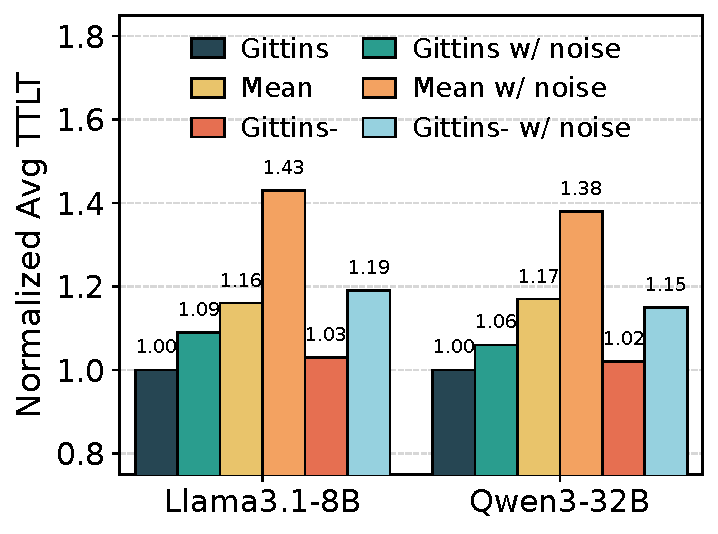
\includegraphics[width=\linewidth]{figures/ablation_on_effect.pdf }
        \caption{不同调度方法对比（含代价噪声注入场景）。}
        \label{fig:ablation_gittins}
    \end{minipage}
    \hfill
    \begin{minipage}[t]{0.47\linewidth}
        \centering
        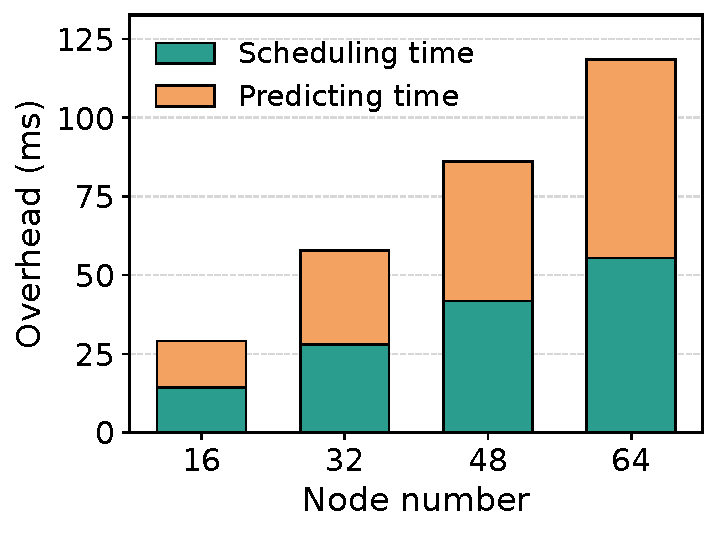
\includegraphics[width=\linewidth]{figures/overhead.pdf}
        \caption{\oursched 在不同规模下的预测与调度开销。}
        \label{fig:overhead}
    \end{minipage}
\end{figure}

\subsection{开销与敏感性分析}
\label{subsec:eval_sensitivity}

本节分析 \oursched 的可扩展性，并对关键超参数进行敏感性研究。
除非特别说明，配置同图~\ref{fig:e2e}。

\phm{可扩展性。}
我们模拟了最多 64 GPU 节点的大规模集群部署。
系统负载（RPS）随集群规模同比增长。
平均每个节点服务 8 RPS，队列中最多缓冲 1000 个请求。
在固定输出长度 1000 token 的设置下，测量预测与调度阶段引入的单请求额外时延。
如图~\ref{fig:overhead} 所示，开销随规模近线性增长。
即便在 64 节点规模下，单请求平均额外时延约 100 ms。
考虑到典型 LLM 推理时延量级通常为秒级到分钟级（见图~\ref{fig:e2e}），该开销可以忽略。
此外，在更大集群中还可部署多个并行调度器进一步降低开销。

\phm{相似度阈值。}
在预测器设计中（第~\ref{subsec:predictor} 节），我们用余弦相似度阈值筛选可参考历史请求。
图~\ref{fig:sensitivity_predictor} 给出了不同阈值下的测试床结果。
可见阈值 0.8 最优：阈值过大导致样本不足（不利于刻画不确定性），阈值过小会引入无关样本污染分布。

\phm{桶大小。}
在第~\ref{subsec:gittins} 节中，我们使用桶大小控制 Gittins 指数刷新频率。
图~\ref{fig:sensitivity_gittins} 展示了不同桶大小下 \oursched 的平均 TTLT。
结果表明桶大小 200 最优（因此设为默认）：桶太小会带来更高优先级计算与重调度开销；桶太大则降低优先级估计精度，二者都会损害整体效率。

\begin{figure}[t]
    \centering
    \subfigure[预测器超参数]{
        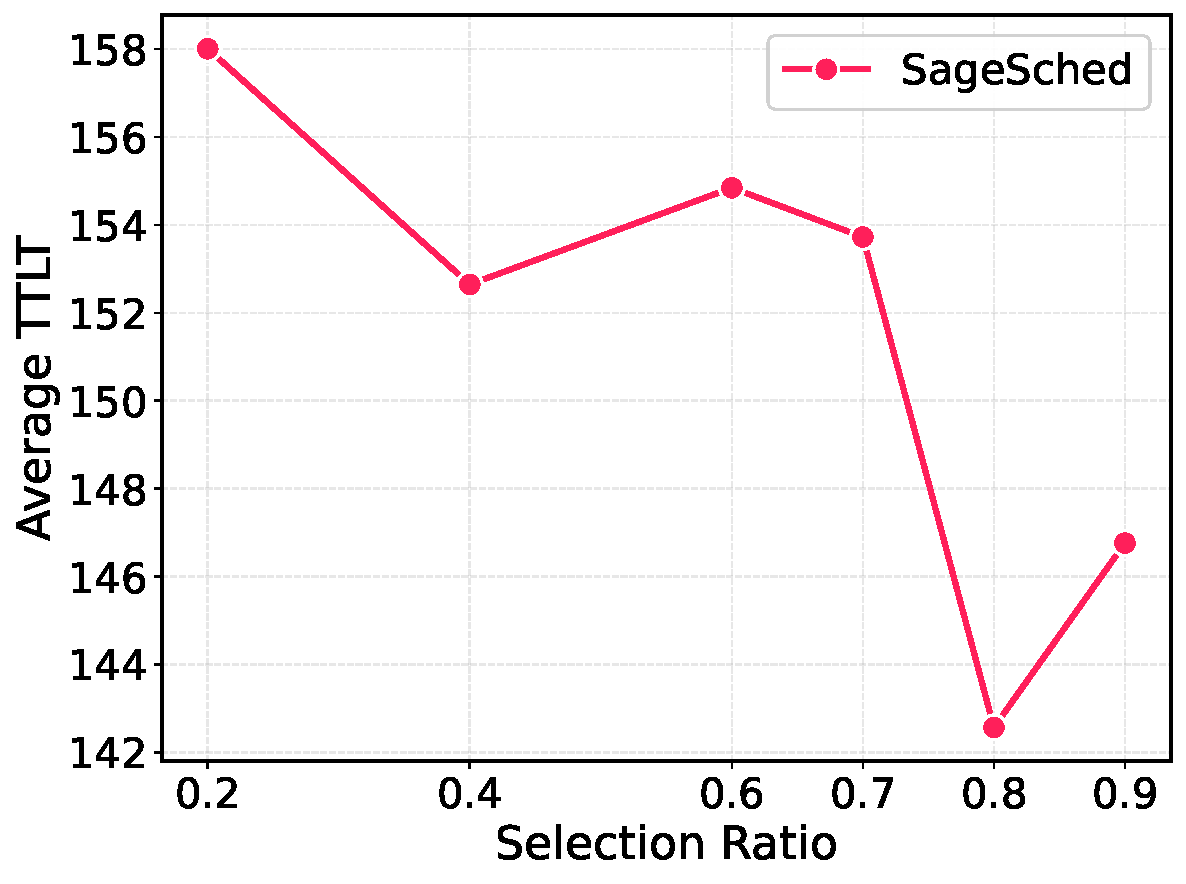
\includegraphics[width=0.45\linewidth]{figures/sensitive_selection.pdf}
        \label{fig:sensitivity_predictor}
    }
    \hfill
    \subfigure[调度器超参数]{
        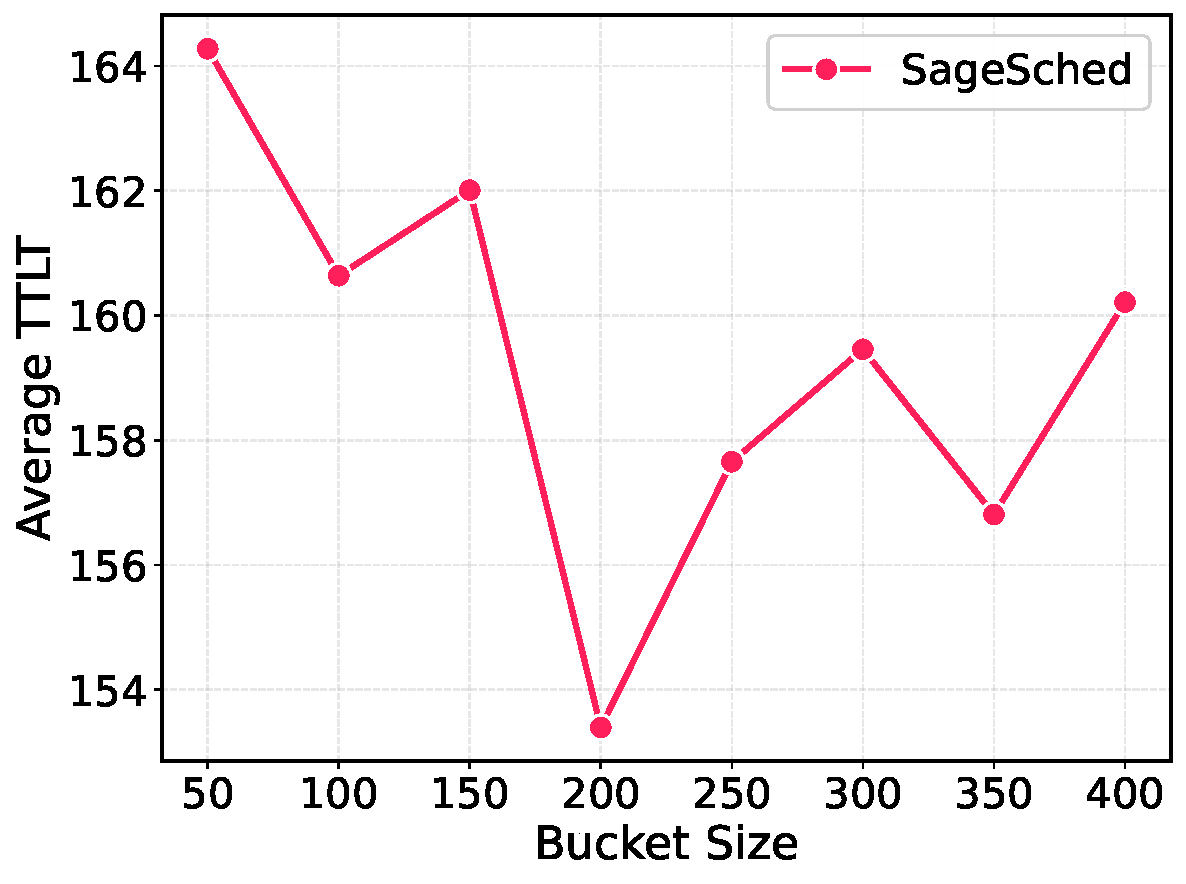
\includegraphics[width=0.45\linewidth]{figures/sensitive_bucket.pdf}
        \label{fig:sensitivity_gittins}
    }
    \vspace{-.1in}
    \caption{\oursched 超参数敏感性分析。}
    \label{fig:sensitivity}
\end{figure}

%!TEX root = main_zh.tex
\section{更多相关工作}
\label{sec:related}

大量研究从互补角度提升 LLM 服务效率，这些方法可与 \oursched 结合使用。
例如，一些工作关注单请求加速：在 token 级别优化~\cite{dao2022flashattention,dao2023flashattention,dettmers2022gpt3,frantar2022gptq,leviathan2023speculative,miao2023specinfer}，或进行部署侧系统优化~\cite{zhong2024distserve,qin2024mooncake,hu2024memserve,hu2024inference,agrawal2024taming}。
另一些工作通过重构 batching 与准入控制机制提升后端利用率~\cite{duan2024muxserve,xiang2025aegaeon}。
此外，由于 KVCache 存储常是主要瓶颈，许多方法也通过压缩或选择性保留来降低 KVCache \emph{大小}~\cite{xiao2023efficient,zhang2023h2o,lee2024infinigen}。
受篇幅限制，详细展开放在附录中。

%!TEX root = main_zh.tex
\section{结论}
\label{sec:conclusion}

本文提出 \oursched，一种面向 LLM 负载\emph{不确定性}与\emph{混合性}特征的高效调度器。
\oursched 通过语义感知历史预测器，以轻量且准确的方式预测输出长度分布；
并在服务代价建模中同时考虑显存与计算瓶颈；
同时采用基于 Gittins 指数的不确定性感知调度策略，以获得更优排队效果。
测试床与仿真实验表明，\oursched 能显著提升端到端效率，TTLT 降幅超过 28.7\%。


\begingroup
\raggedright
\bibliography{main}
\bibliographystyle{icml2026}
\endgroup

%%%%%%%%%%%%%%%%%%%%%%%%%%%%%%%%%%%%%%%%%%%%%%%%%%%%%%%%%%%%%%%%%%%%%%%%%%%%%%%
%%%%%%%%%%%%%%%%%%%%%%%%%%%%%%%%%%%%%%%%%%%%%%%%%%%%%%%%%%%%%%%%%%%%%%%%%%%%%%%
% APPENDIX
%%%%%%%%%%%%%%%%%%%%%%%%%%%%%%%%%%%%%%%%%%%%%%%%%%%%%%%%%%%%%%%%%%%%%%%%%%%%%%%
%%%%%%%%%%%%%%%%%%%%%%%%%%%%%%%%%%%%%%%%%%%%%%%%%%%%%%%%%%%%%%%%%%%%%%%%%%%%%%%
\newpage
\appendix
\onecolumn

\section{相关工作完整版}
我们的工作聚焦于在不确定且混合（计算--显存）需求下进行\emph{请求级调度}；以下研究方向大多与 \oursched 正交，可组合使用。

\phm{LLM 推理加速。}
大量工作旨在降低 LLM 推理的\emph{单 token}计算与显存代价。
在算子/内核层面，FlashAttention 与 FlashAttention-2 通过重组注意力计算改善内存局部性并减少冗余读写，实现更快且更省显存的精确注意力~\cite{dao2022flashattention,dao2023flashattention}。
模型压缩与低比特量化也可在维持精度前提下降低内存占用，例如 INT8 矩阵乘与 Transformer 权重后训练量化~\cite{dettmers2022gpt3,frantar2022gptq}。
近期解码加速方法广泛利用\emph{投机执行}：投机解码先由快速草稿模型提出多个 token，再由目标模型验证~\cite{leviathan2023speculative}；后续系统通过 token-tree 验证与在线机制进一步提升效率~\cite{miao2023specinfer,liu2023online}。

除 token 级优化外，系统层设计也在改进端到端流水线。
Prefill--Decode 解耦将吞吐导向的 prefill 与时延敏感的 decode 分离，并重构多设备间 KVCache 放置~\cite{zhong2024distserve,qin2024mooncake,hu2024memserve,hu2024inference}；
chunked-prefill 则通过长上下文 prefill 与 decode 重叠并提升缓存复用，更好平衡吞吐与时延~\cite{agrawal2024taming,hu2024inference}。

这些技术提升的是“每个请求如何更快执行”；\oursched 与之互补，关注在资源受限且请求长度变化时“下一步该服务哪个请求”。

\phm{LLM 服务架构与多路复用。}
许多系统通过重构批处理、准入控制和多租户资源共享来提升后端利用率。
基础服务框架（如 Orca 风格连续批处理，以及 vLLM、SGLang 等现代引擎）强调设备高利用与高效 KVCache 管理~\cite{yu2022orca,kwon2023efficient,zheng2024sglang}。
在多模型、多租户场景中，近期工作探索更细粒度的复用与资源池化：MuxServe 支持时空复用以在共享 GPU 上协同多类 LLM 负载~\cite{duan2024muxserve}；Aegaeon 面向并发 LLM 服务提出有效的 GPU 池化机制~\cite{xiang2025aegaeon}。

这些系统主要解决模型/租户间资源共享与放置问题；\oursched 则聚焦后端内部在服务时长不确定条件下的请求排序，可作为每 GPU（或每资源池）的调度模块接入。

\phm{LLM 请求调度与公平性。}
越来越多工作研究请求调度以缓解队首阻塞并优化尾时延。
生产引擎通常从 FCFS 起步，虽然简单，但在请求长度异构场景下会明显恶化 TTLT~\cite{kwon2023efficient,zheng2024sglang}。
FastServe 用 MLFQ 近似 SRPT，通过周期性降级优先级换取时延收益，但伴随额外抢占开销~\cite{wu2023fast}。
更新的调度器采用\emph{预测后排序}范式：$S^3$ 通过微调小模型估计生成长度~\cite{jin2023s}，PO 让 LLM 预估自身输出长度~\cite{po}，SSJF 用代理模型预测输出长度并近似 SJF~\cite{qiu2024efficient}，学习排序方法预测相对长度顺序而非绝对值~\cite{fu2024efficient}。
基于嵌入的调度器还会利用 LLM 中间层特征改进优先级估计~\cite{shahout2024don}。
同时，公平性研究从效率与服务区分度之间张力出发提出公平调度机制~\cite{sheng2024fairness}；Llumnix 则引入运行时条件实现动态重排~\cite{sun2024llumnix}。

与上述工作相比，\oursched 的差异主要有三点：
(i) 采用\emph{分布级}（而非点估计）输出长度感知，避免单值预测脆弱性；
(ii) 建模由 KVCache 增长带来的\emph{计算--显存混合代价}，而非仅用输出长度；
(iii) 在抢占决策中显式考虑 I/O 影响，以避免过度交换同时保持优先级修正能力。

\phm{KVCache 管理与长上下文服务。}
由于解码阶段每步都要关注全部历史 token，KVCache 往往是主要显存瓶颈。
PagedAttention（vLLM 中实现）通过分页式 KV 分配降低碎片并提高显存效率~\cite{kwon2023efficient}。
除分配方式外，也有大量工作通过压缩或选择性保留降低 KVCache \emph{体积}：attention sink 通过稳定注意力模式支持高效流式推理~\cite{xiao2023efficient}；heavy-hitter 方法在显存受限时保留最关键 token 近似全注意力~\cite{zhang2023h2o}。
近期还有跨时间动态管理方案：InfiniGen 提出高效生成推理的动态 KVCache 管理~\cite{lee2024infinigen}；KIVI 通过无需调参的非对称 2-bit KV 量化降低显存与带宽压力~\cite{liu2024kivi}。

这些进展提升了可并发度和单步效率；\oursched 与其正交，并可通过基于代价分布的优先级进一步降低 TTLT，从而更充分利用 KVCache 增长与资源竞争信息。

%%%%%%%%%%%%%%%%%%%%%%%%%%%%%%%%%%%%%%%%%%%%%%%%%%%%%%%%%%%%%%%%%%%%%%%%%%%%%%%
%%%%%%%%%%%%%%%%%%%%%%%%%%%%%%%%%%%%%%%%%%%%%%%%%%%%%%%%%%%%%%%%%%%%%%%%%%%%%%%


\end{document}
